\chapter{译码算法对比}\label{chap:decoder}

\section{对比目标与统一仿真条件}

\subsection{译码算法对比目标}

在编码方案已经确定的基础上，固定业务输入、编码配置和加性高斯白噪声（Additive White Gaussian Noise，AWGN）条件，在各编码族内部更换译码实现，以比较译码器对可靠性与实现代价的共同影响。可靠性采用比特错误率（Bit Error Rate，BER）和帧错误率（Frame Error Rate，FER）表征；实现代价分为算法操作规模、译码器存储开销和当前软件平台上的实测译码时间。平均译码时间与最大观测译码时间是本章的主要时间指标，P95、P99、迭代次数、提前停止率、首输出时延和决策时延用于补充描述尾部波动、收敛行为与流式输出特性。

表\ref{tab:s6-control-variables}给出三类比较的控制边界。卷积码硬、软判决是在编码器、码率和码长不变时更换分支度量输入，因而最接近单一译码因素对比；LDPC的BP与归一化最小和（Normalized Min-Sum，NMS）共享逐帧输入及噪声，实现了严格配对；BCH两条路线同时改变码型、发送长度、纠错能力、分块组织和译码器，因此只能解释为两套完整BCH实现方案的综合比较。

\begin{table}[htbp]
  \centering
  \scriptsize
  \caption{S6译码算法对比的控制变量与变化变量}
  \label{tab:s6-control-variables}
  \setlength{\tabcolsep}{2.0pt}
  \begin{tabular}{p{0.09\textwidth}p{0.18\textwidth}p{0.18\textwidth}p{0.17\textwidth}p{0.17\textwidth}p{0.10\textwidth}}
    \toprule
    编码类型 & 冻结条件 & 变化条件 & 对比对象 & 主要指标 & 可比性说明 \\
    \midrule
    BCH & 200 bit业务输入、BPSK、AWGN、硬判决与统计规则 & 码型、分块、发送长度、纠错能力及译码器 & BCH-S200与BCH-B200 & BER、FER、操作、内存、时间 & 完整方案对比，不能作纯译码因果归因 \\
    卷积码 & 300 bit输入、$R=300/612$、相同网格及Viterbi骨架 & 硬判决或浮点软判决；整块或连续组织 & 8种组织与判决组合 & BER、FER、ACS、回溯、内存、时间与输出时延 & 数据复用自既有正式试验，非S6 strict pair-stop重跑 \\
    LDPC & 同一300 bit载荷、N560码字、LLR、图结构、迭代上限与停止规则 & 校验节点更新算法 & 分层BP与分层NMS & BER、FER、迭代、操作、内存、时间 & 逐信噪比共享载荷、码字和LLR \\
    \bottomrule
  \end{tabular}
\end{table}

\subsection{统一仿真条件}

三类结果均采用幅度为$\pm1$的二进制相移键控（Binary Phase Shift Keying，BPSK），以符号信噪比$E_s/N_0$作为主横轴。实值AWGN方差为
\begin{equation}
  \sigma^2=\frac{1}{2\times10^{(E_s/N_0)/10}} .
\end{equation}
由码率换算的$E_b/N_0$只用于模块内部辅助记录，不能替代本章图中的$E_s/N_0$口径。各工作点从$-5$ dB到$10$ dB，步长为$0.5$ dB。每点至少运行1000帧，达到目标200个错误帧后可停止，最多运行50000帧。高信噪比处未观测到错误的原始零值仍保留在数据中，但不在对数坐标上伪造非零点，也不参与FER门限外推。

\begin{table}[htbp]
  \centering
  \small
  \caption{S6译码算法比较的公共仿真条件}
  \label{tab:s6-common-settings}
  \begin{tabular}{p{0.24\textwidth}p{0.66\textwidth}}
    \toprule
    项目 & 设置 \\
    \midrule
    调制与信道 & BPSK；实值AWGN \\
    主信噪比口径 & $E_s/N_0$，范围$-5\sim10$ dB，步长$0.5$ dB，共31点 \\
    停止条件 & 每点至少1000帧；目标错误帧数200；每点最多50000帧 \\
    随机与噪声规则 & 按帧索引确定性生成信息与标准高斯母噪声；同一编码族的对比译码器共享规定输入。BCH全局种子为20260804；卷积码载荷与噪声种子分别为2026072001和2026072904 \\
    可靠性判据 & 恢复载荷逐比特比较；任一载荷比特错误即记为错误帧 \\
    计时单位 & 微秒/帧；计时范围仅覆盖相应C++译码调用 \\
    已记录运行环境 & Windows 11、Intel Core i5-14400F、GNU C++ 15.2.0、C++17、Release、单线程、\texttt{steady\_clock} \\
    \bottomrule
  \end{tabular}
\end{table}

\subsection{复杂度与时延定义}

本章把实现代价拆分为三个互不替代的维度。算法操作规模记录译码过程中发生的结构化事件，适合在同一编码族和同一计数口径内比较；存储开销记录由类型和缓冲区规模推导的译码器内存模型，不是完整进程驻留集；软件译码时间是当前C++实现、编译配置和处理器上的墙钟测量值，不代表硬件绝对时延。BCH的异或、有限域运算，卷积码的加比选（Add--Compare--Select，ACS），以及LDPC的双曲函数、比较和最小值操作具有不同语义与成本，不能简单相加成跨编码族的“统一总复杂度”。

\begin{table}[htbp]
  \centering
  \scriptsize
  \caption{本章译码复杂度与时延指标定义}
  \label{tab:s6-metric-definitions}
  \setlength{\tabcolsep}{2.2pt}
  \begin{tabular}{p{0.17\textwidth}p{0.23\textwidth}p{0.30\textwidth}p{0.20\textwidth}}
    \toprule
    维度 & 指标与单位 & 统计含义 & 使用限制 \\
    \midrule
    算法操作规模 & BCH综合征、查表、BM、Chien和有限域事件；卷积码ACS与回溯；LDPC消息更新及节点运算，单位为事件/帧 & 由译码源码中的结构化计数器累计，同族内反映计算结构与工作量 & 不同操作不能按一次等价成本跨族相加 \\
    存储开销 & 译码器内存与峰值工作区，字节 & 静态表、对象、消息、路径度量、回溯或工作缓冲的模型值 & 不含完整进程RSS，静态表与临时工作区须分开解释 \\
    平均译码时间 & 每点平均值及跨信噪比帧加权平均值，$\mu$s/帧 & 计时器包围译码调用；汇总值按各点帧数加权 & 依赖处理器、编译器、实现和运行状态 \\
    尾部与最大时间 & P95、P99和最大观测值，$\mu$s/帧 & P95/P99来自相应正式图数据；最大值为全部工作点的观测最大值 & 最大值反映观测尖峰，不等同于硬实时上界 \\
    流式输出时延 & 首输出和决策时延，符号 & 由在线调度和窗口结构决定 & 不是CPU译码时间，不能代替平均或最大墙钟时间 \\
    \bottomrule
  \end{tabular}
\end{table}

\begin{figure}[htbp]
  \centering
  \fbox{\begin{minipage}[c][0.18\textheight][c]{0.86\textwidth}
    \centering\large 译码算法比较的统一仿真流程\\[0.8em]
    \small 随机信息比特 $\rightarrow$ 冻结编码器 $\rightarrow$ BPSK $\rightarrow$ AWGN\\
    $\rightarrow$ 共享接收样本 $\rightarrow$ 译码算法A/译码算法B\\
    $\rightarrow$ BER、FER、操作规模、存储与软件译码时间
  \end{minipage}}
  \caption{S6译码算法比较统一仿真流程}
  \label{fig:s6-flow-placeholder}
\end{figure}

\section{BCH不同译码实现方案对比}

\subsection{比较对象与公平性边界}

BCH-S200把200 bit载荷补入9个零后分为19组，每组采用BCH(15,11,1)，实际发送285 bit，码率为$200/285=0.7018$，译码器按综合征查询单错位置表。BCH-B200采用缩短BCH(255,207)，从母码信息区缩短7 bit，实际发送248 bit，码率为$200/248=0.8065$，保证纠错能力$t=6$，译码流程由综合征求值、Berlekamp--Massey（BM）迭代和Chien搜索组成。

表\ref{tab:s6-bch-boundary}明确了因果边界：两种方案除了译码方法，还同时改变了码型、分组数、发送长度、码率和纠错能力。因此，以下BER与FER差异只能归属于本项目既定的两类完整BCH编译码实现，不能表述为“BM本身必然优于查表”。

\begin{table}[htbp]
  \centering
  \scriptsize
  \caption{BCH两类译码实现及比较边界}
  \label{tab:s6-bch-boundary}
  \setlength{\tabcolsep}{2.0pt}
  \begin{tabular}{p{0.10\textwidth}c p{0.16\textwidth}c c c c p{0.16\textwidth}p{0.13\textwidth}}
    \toprule
    方案 & 载荷 & BCH码型 & 分组数 & 发送长度 & 码率 & 纠错能力 & 译码器 & 比较说明 \\
    \midrule
    BCH-S200 & 200 & BCH(15,11,1) & 19 & 285 & 0.7018 & 每组1 bit & 综合征查表 & 末组填充9 bit，短分组固定结构 \\
    BCH-B200 & 200 & 缩短BCH(255,207) & 1 & 248 & 0.8065 & 整块6 bit & BM与Chien搜索 & 缩短7 bit，整块代数译码 \\
    \bottomrule
  \end{tabular}
\end{table}

\subsection{BER与FER}

图\ref{fig:s6-bch-reliability}表明，两种方案在低$E_s/N_0$区均处于高错误率区，进入瀑布区后BCH-B200的BER和FER曲线更早下降。依据相邻真实非零FER点的$\log_{10}(\mathrm{FER})$线性插值，FER为0.1时，BCH-S200与BCH-B200所需$E_s/N_0$分别为4.667 dB和3.612 dB，完整整块方案节省1.056 dB；FER为0.01时，两者分别为6.040 dB和4.369 dB，差值增至1.671 dB。高信噪比处的零错误点仅表示有限样本中未观测到错误：S200有4个零BER/FER点，B200有9个，图中没有对这些点进行对数伪值替换或外推。

\begin{figure}[p]
  \centering
  \begin{minipage}{0.92\textwidth}\centering
    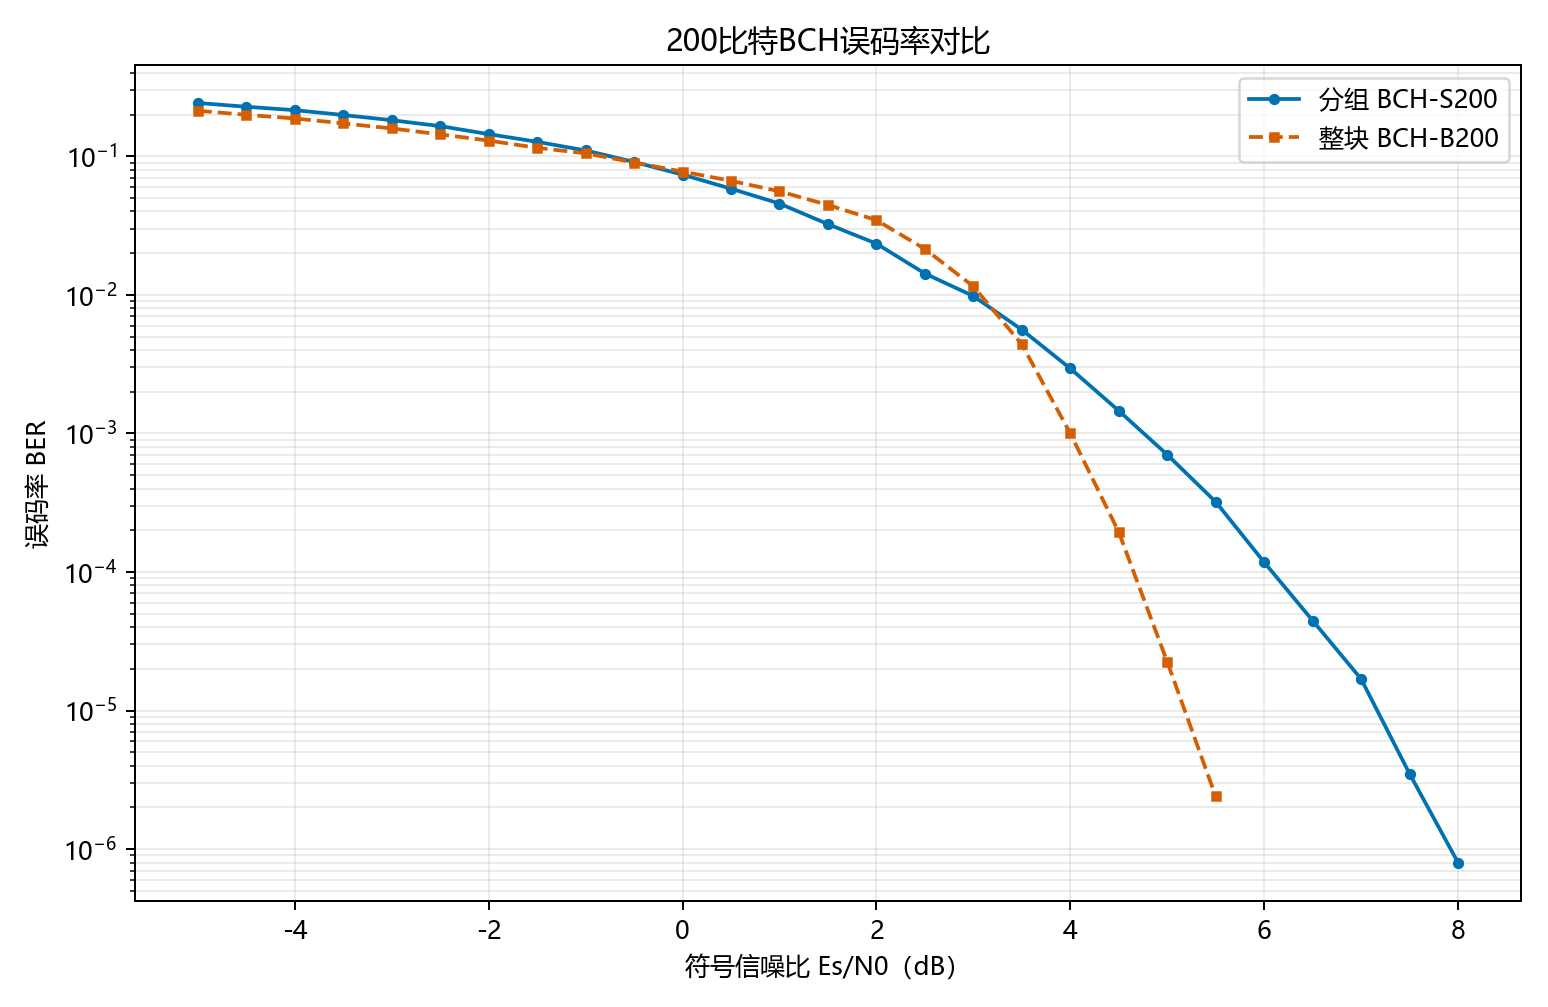
\includegraphics[width=0.90\linewidth]{../Task/Comparison/S6/results/summary/figures/bch_01_ber/figure.png}\\[-0.2em]
    \small（a）比特错误率
  \end{minipage}\par\medskip
  \begin{minipage}{0.92\textwidth}\centering
    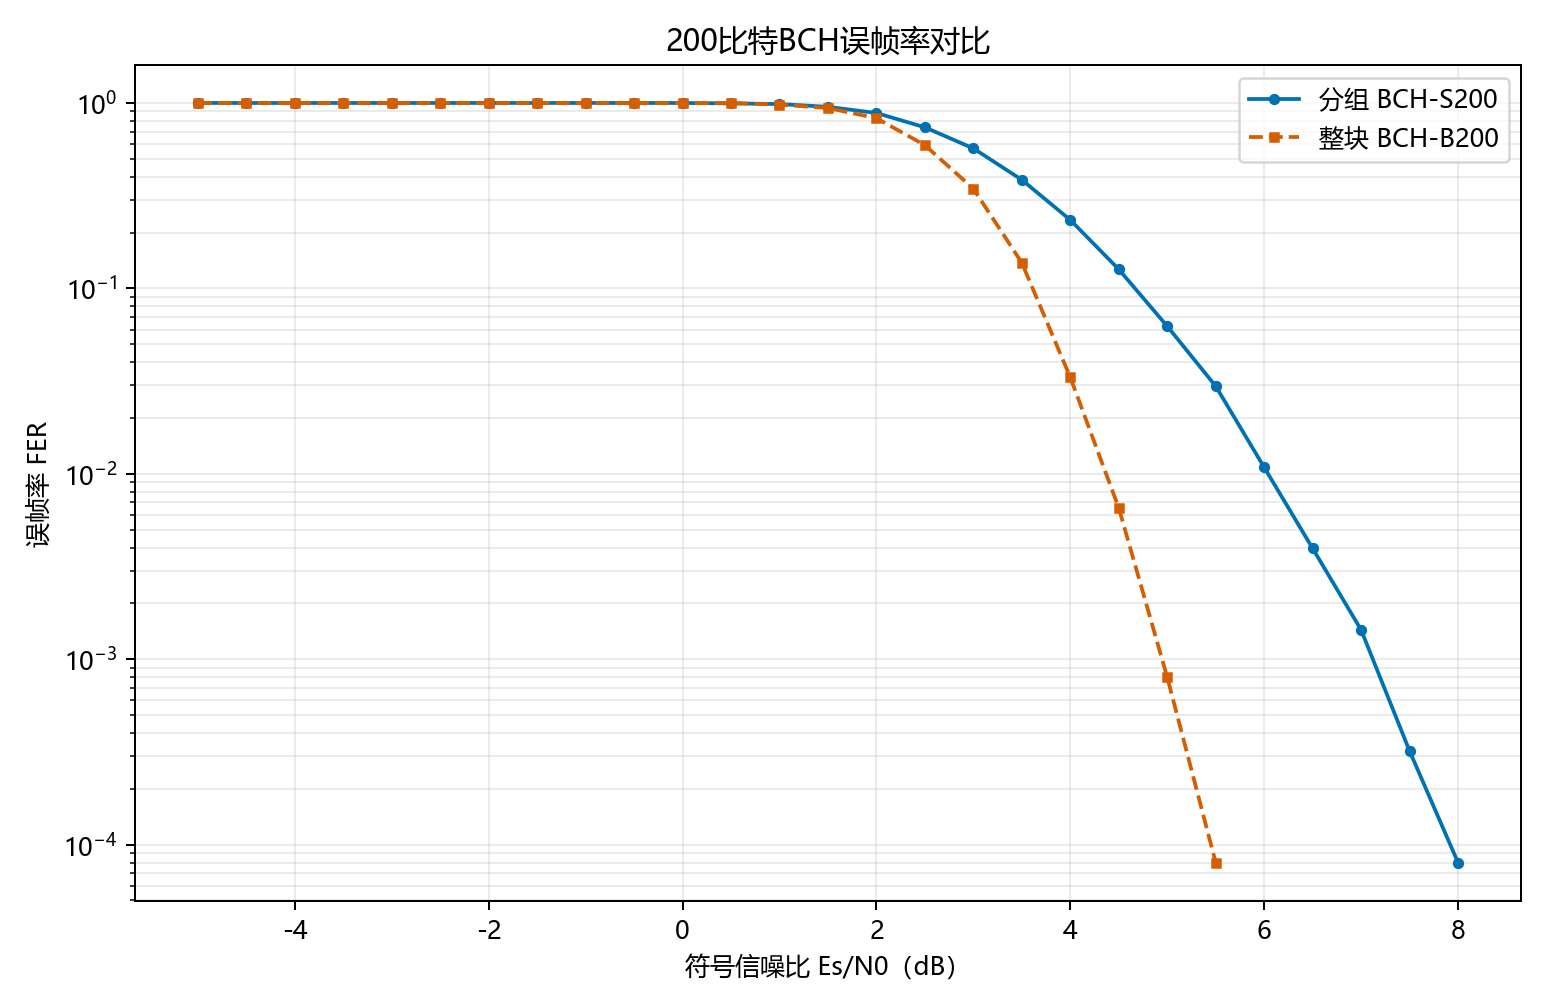
\includegraphics[width=0.90\linewidth]{../Task/Comparison/S6/results/summary/figures/bch_02_fer/figure.png}\\[-0.2em]
    \small（b）帧错误率
  \end{minipage}
  \caption{BCH两类实现的BER与FER}
  \label{fig:s6-bch-reliability}
\end{figure}

\subsection{计算结构与操作统计}

BCH-S200对19个短子块计算综合征；综合征非零时执行位测试、查表、候选比特翻转和译后检查。图\ref{fig:s6-bch-operations}显示，其网格均值为每帧26.92次综合征计算、296.16次综合征位测试和7.92次查表；后三类纠错相关操作会随信道改善而减少。BCH-B200每帧固定完成3060次综合征求值，随后执行BM迭代和Chien位置测试，网格均值分别为8.64次和183.07次，同时伴随约4117.52次有限域加法、1143.42次有限域乘法和3.64次有限域除法。该结构解释了整块方案更重的有限域计算负担，但这些事件不是等价指令，不能用计数总和直接换算处理器周期。

\begin{figure}[p]
  \centering
  \begin{minipage}{0.92\textwidth}\centering
    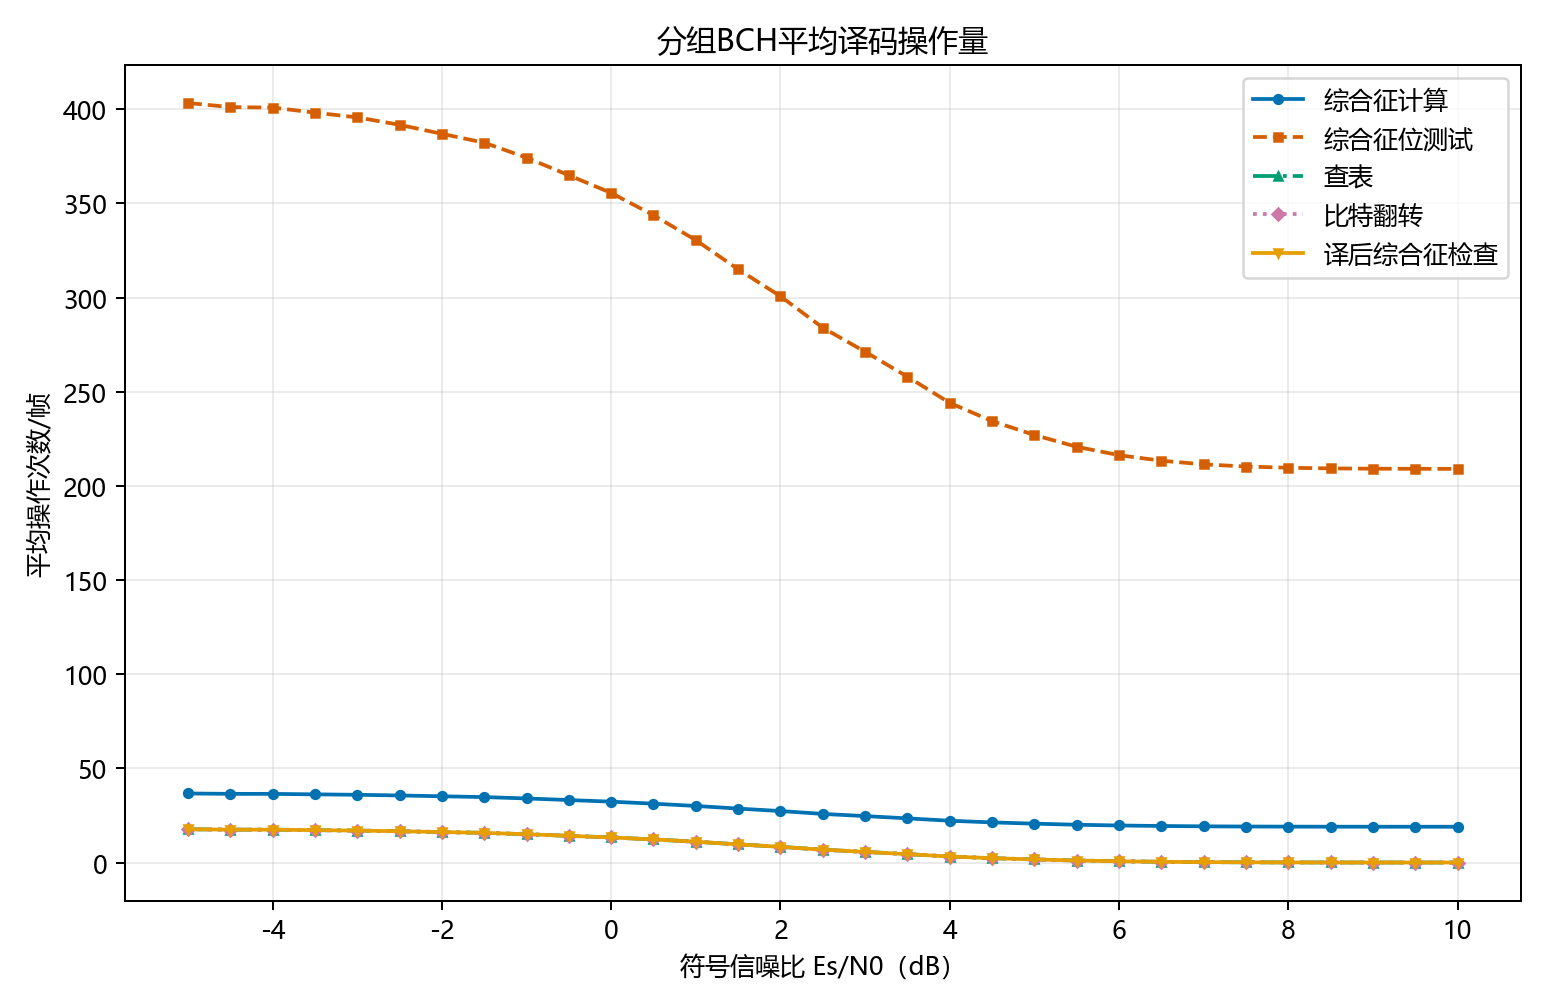
\includegraphics[width=0.72\linewidth]{../Task/Comparison/S6/results/summary/figures/bch_03_segmented_operations/figure.png}\\[-0.2em]
    \small（a）分组查表译码操作
  \end{minipage}\par\medskip
  \begin{minipage}{0.92\textwidth}\centering
    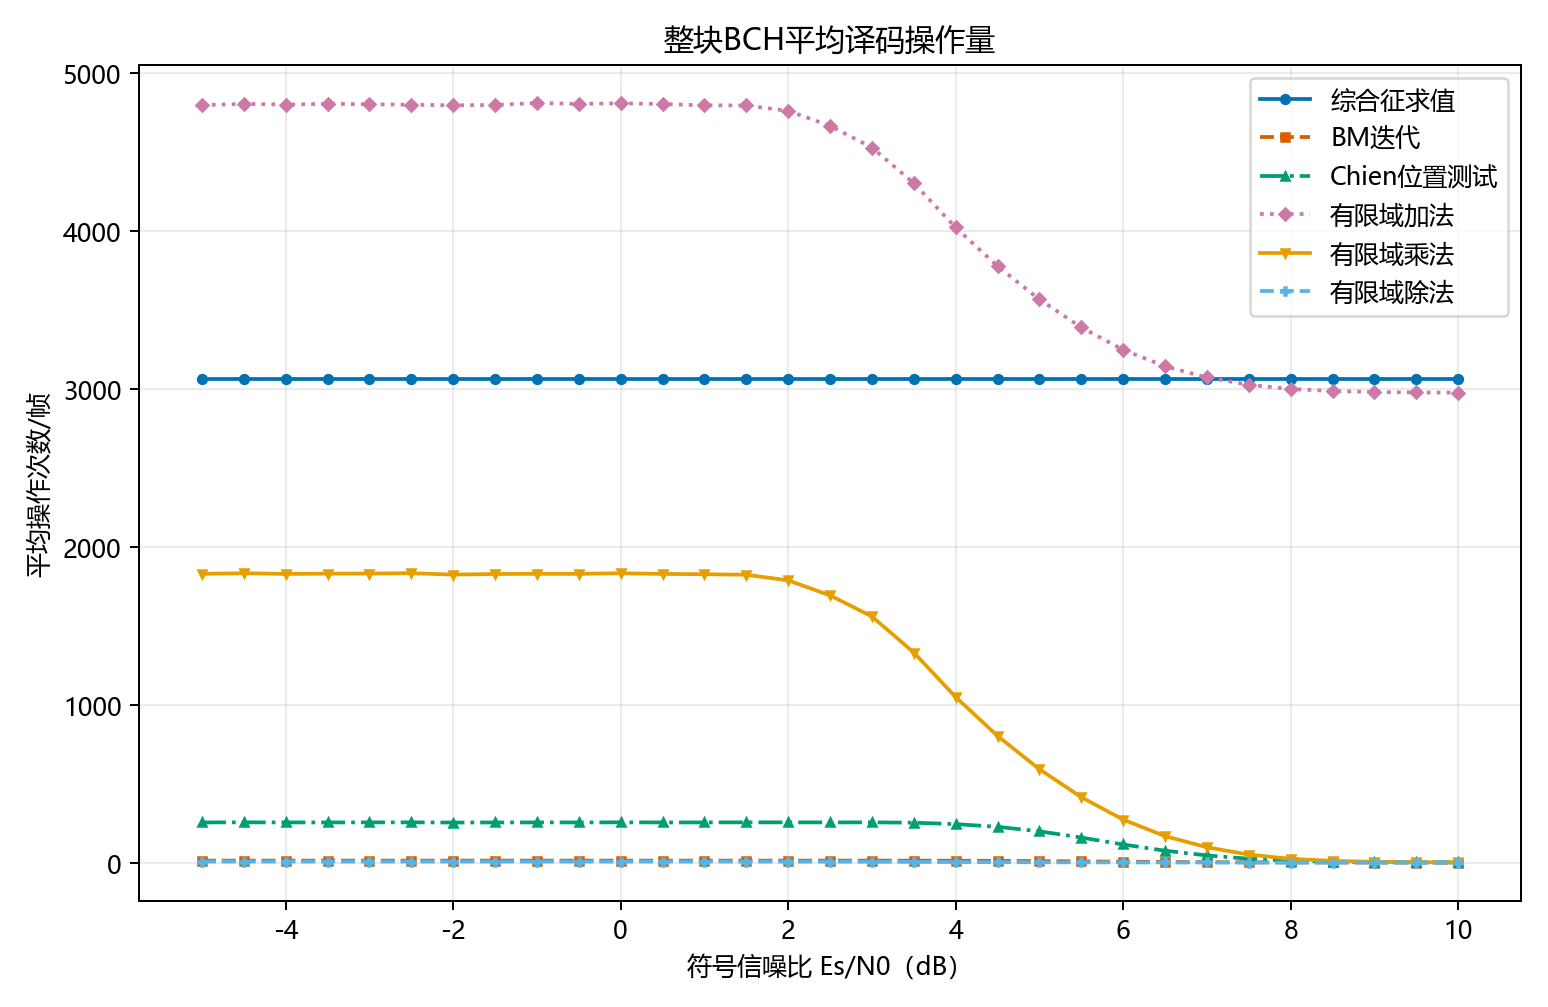
\includegraphics[width=0.72\linewidth]{../Task/Comparison/S6/results/summary/figures/bch_04_block_operations/figure.png}\\[-0.2em]
    \small（b）整块代数译码操作
  \end{minipage}\par\medskip
  \begin{minipage}{0.92\textwidth}\centering
    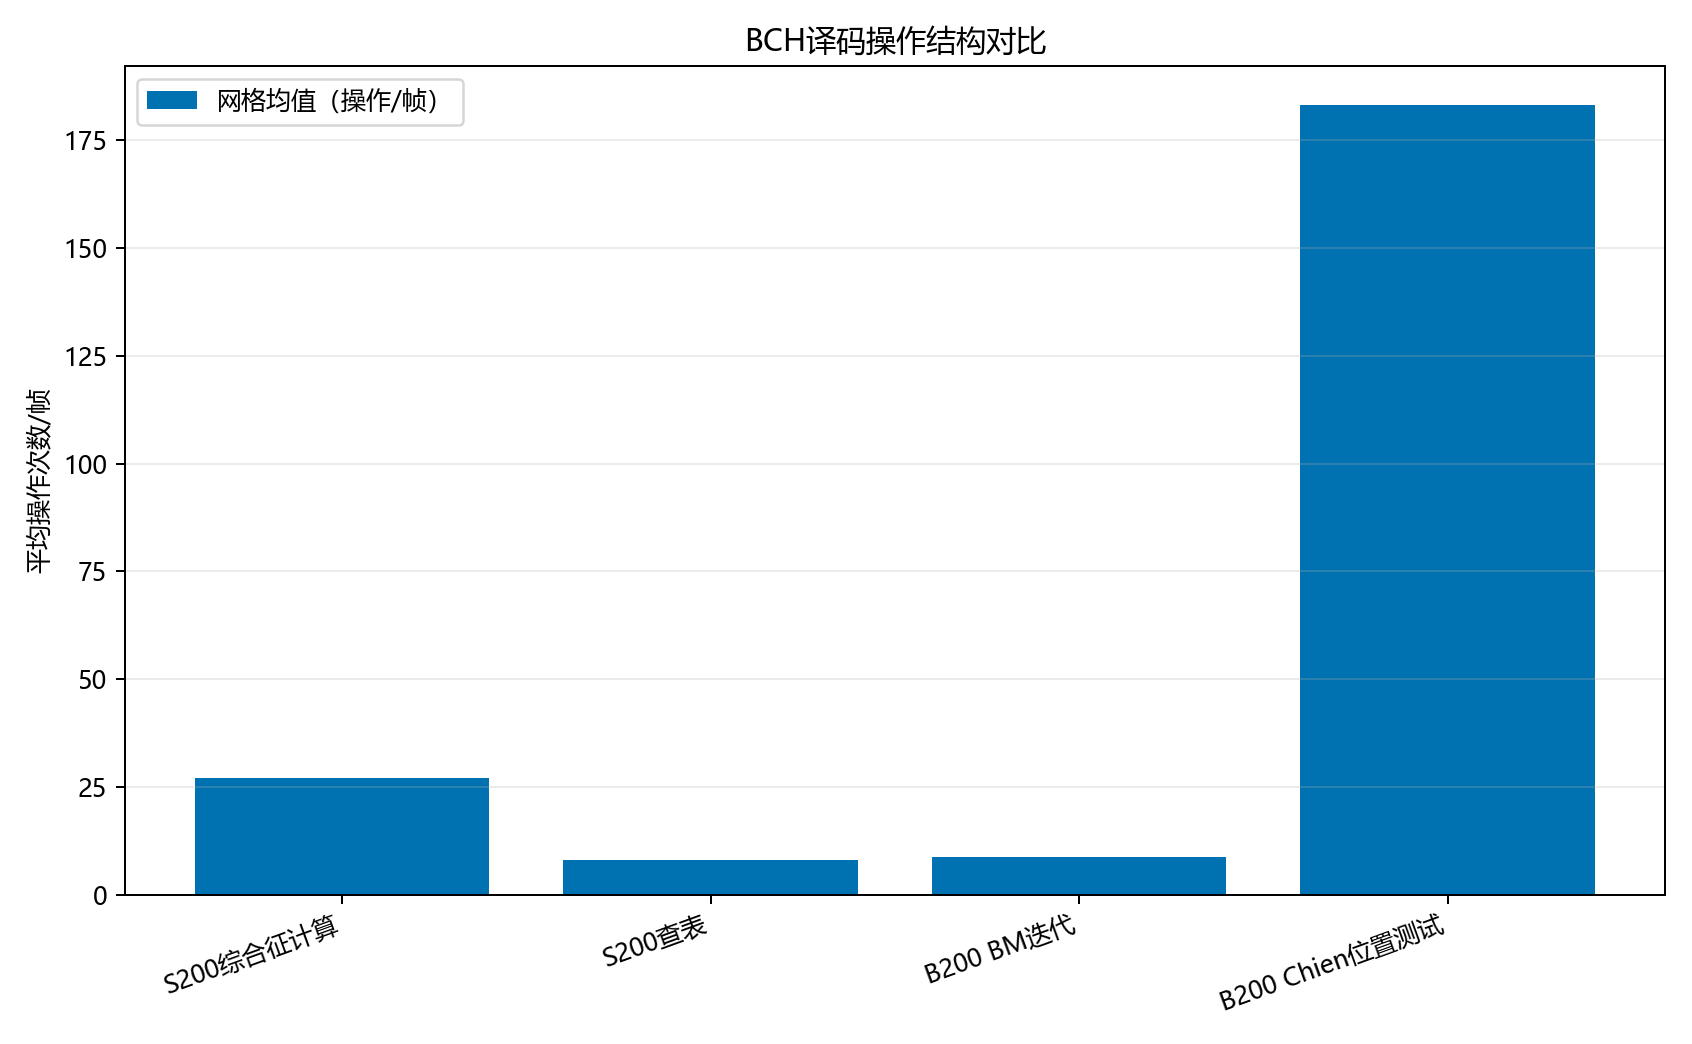
\includegraphics[width=0.68\linewidth]{../Task/Comparison/S6/results/summary/figures/bch_05_operation_structure/figure.png}\\[-0.2em]
    \small（c）主要操作结构的网格均值
  \end{minipage}
  \caption{BCH译码计算结构与操作统计}
  \label{fig:s6-bch-operations}
\end{figure}

\subsection{存储与软件译码时间}

图\ref{fig:s6-bch-memory}中的译码器内存由静态表、对象、输入输出缓冲和工作区按类型与数量建模。BCH-S200总内存为1580 byte，峰值工作区779 byte；BCH-B200总内存为2408 byte，峰值工作区810 byte。整块方案总内存增加828 byte，即52.4\%，主要来自有限域表和代数译码状态；峰值工作区仅增加31 byte。该口径不包含完整进程驻留内存，静态表与临时工作区也未混为同一概念。

\begin{figure}[htbp]
  \centering
  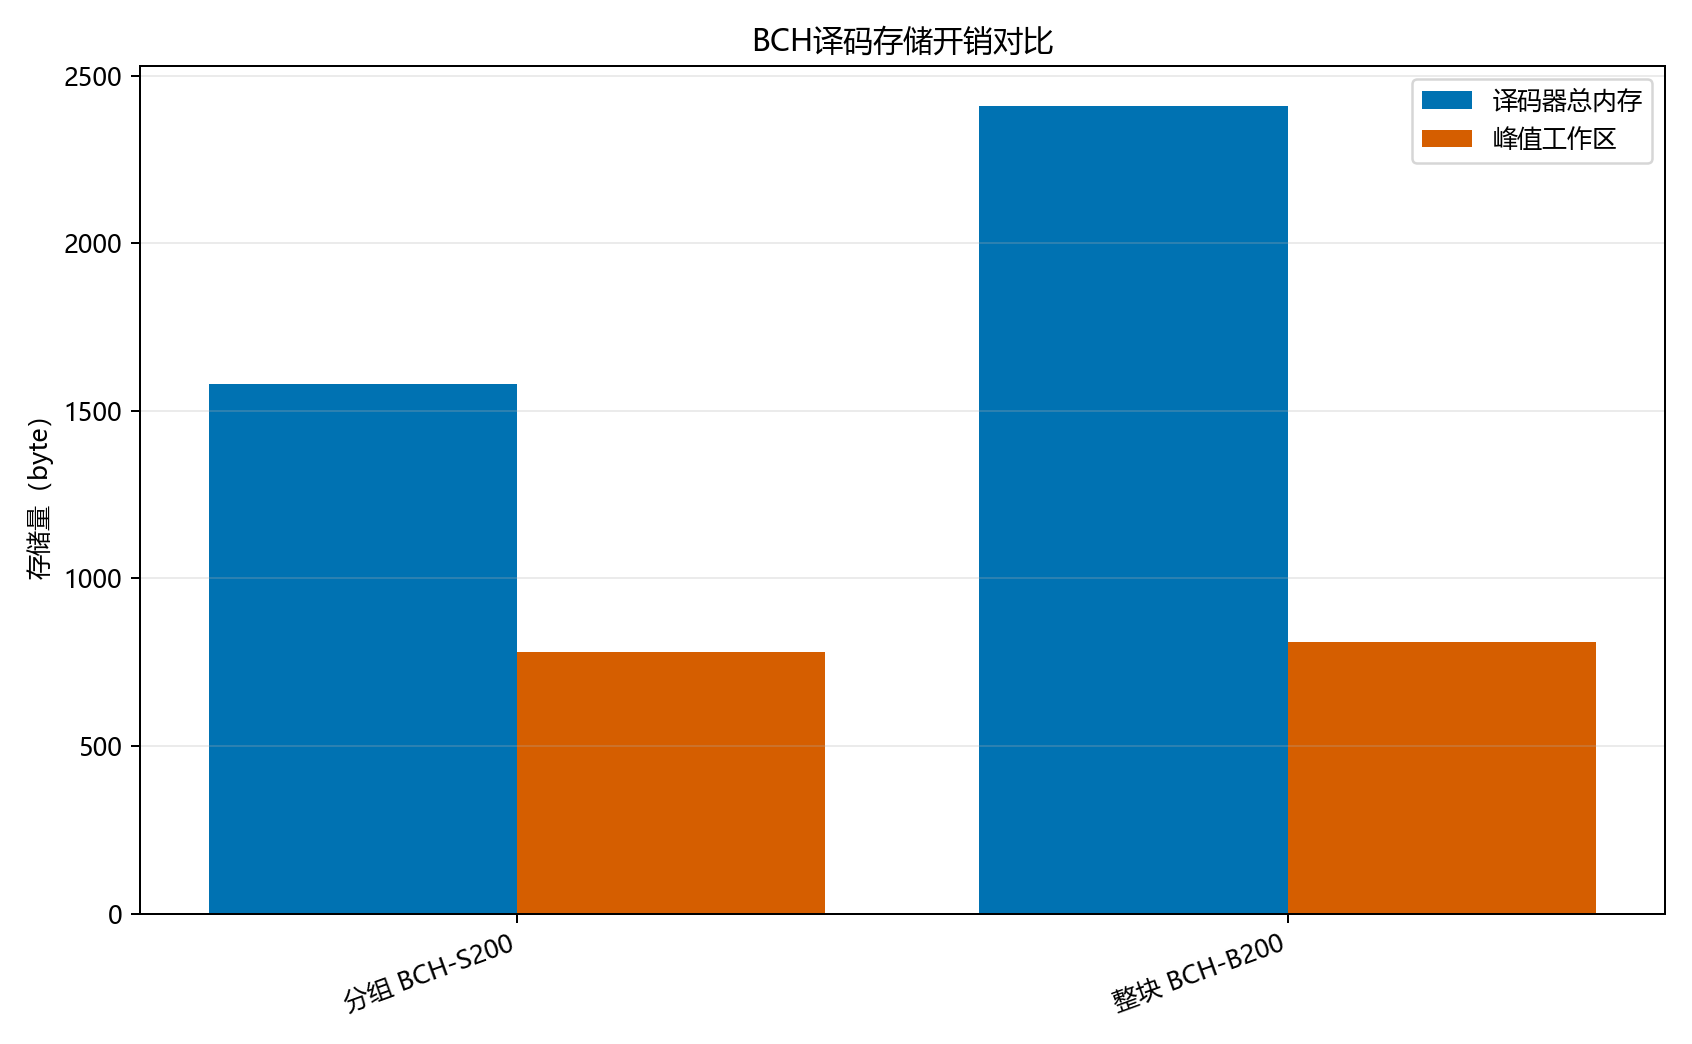
\includegraphics[width=0.90\textwidth]{../Task/Comparison/S6/results/summary/figures/bch_06_memory/figure.png}
  \caption{BCH译码器存储开销}
  \label{fig:s6-bch-memory}
\end{figure}

图\ref{fig:s6-bch-time}覆盖平均、P95、P99和最大观测软件译码时间。按全部信噪比点的帧数加权，S200与B200的平均译码时间分别为10.217~$\mu$s和17.415~$\mu$s，整块方案增加70.5\%；最大观测值分别为25240.3~$\mu$s和27491.4~$\mu$s，增加8.9\%。逐点P95范围分别为10.90--26.53~$\mu$s和15.40--33.52~$\mu$s。P95和P99来自对应正式图数据，而不是不含这两列的汇总表。最大观测值受操作系统调度等影响，只能用于描述当前测量中的尖峰，不能解释为硬实时上界。

\begin{figure}[p]
  \centering
  \begin{minipage}{0.49\textwidth}\centering
    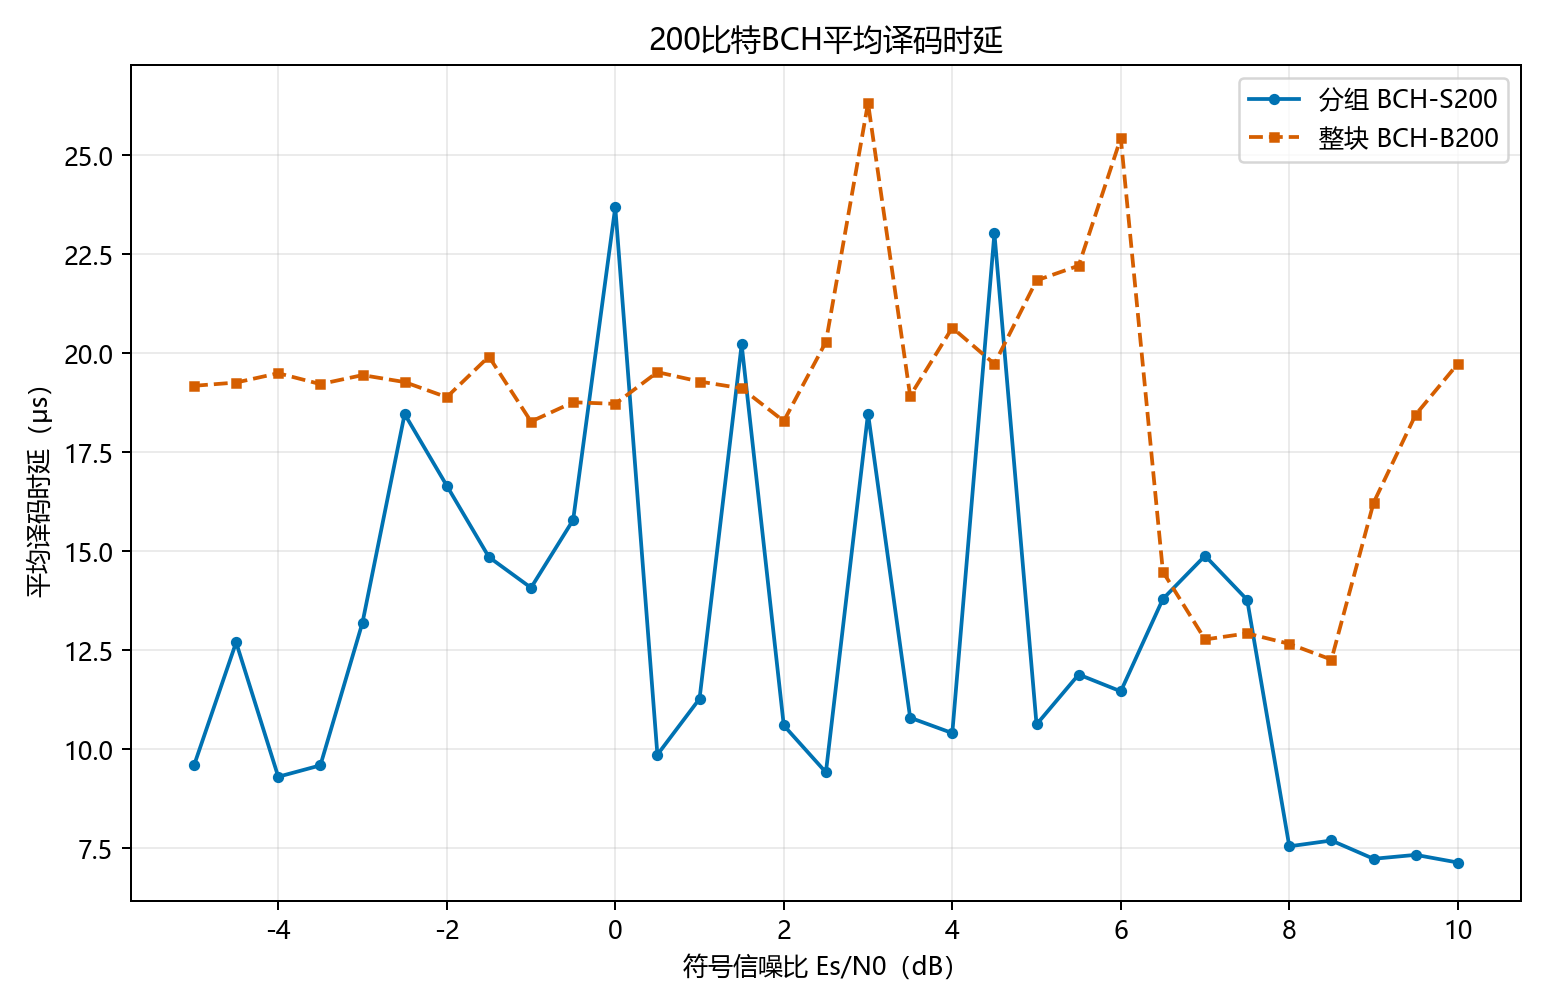
\includegraphics[width=0.98\linewidth]{../Task/Comparison/S6/results/summary/figures/bch_07_avg_time/figure.png}\\[-0.2em]\small（a）平均时间
  \end{minipage}\hfill
  \begin{minipage}{0.49\textwidth}\centering
    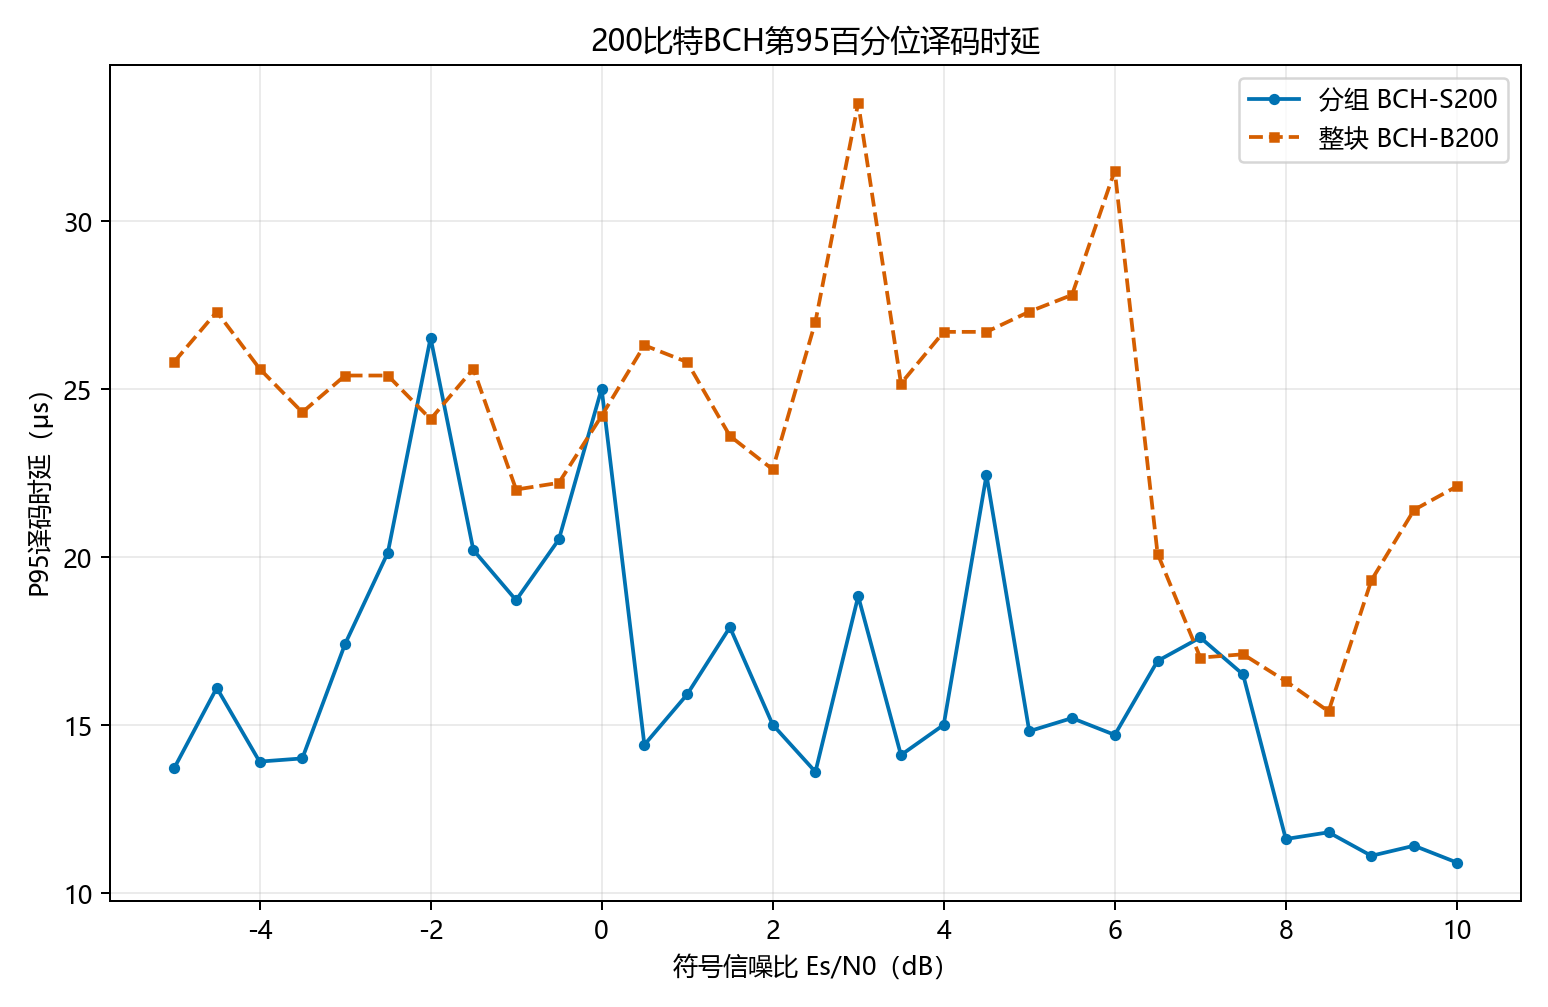
\includegraphics[width=0.98\linewidth]{../Task/Comparison/S6/results/summary/figures/bch_08_p95_time/figure.png}\\[-0.2em]\small（b）P95时间
  \end{minipage}\par\medskip
  \begin{minipage}{0.49\textwidth}\centering
    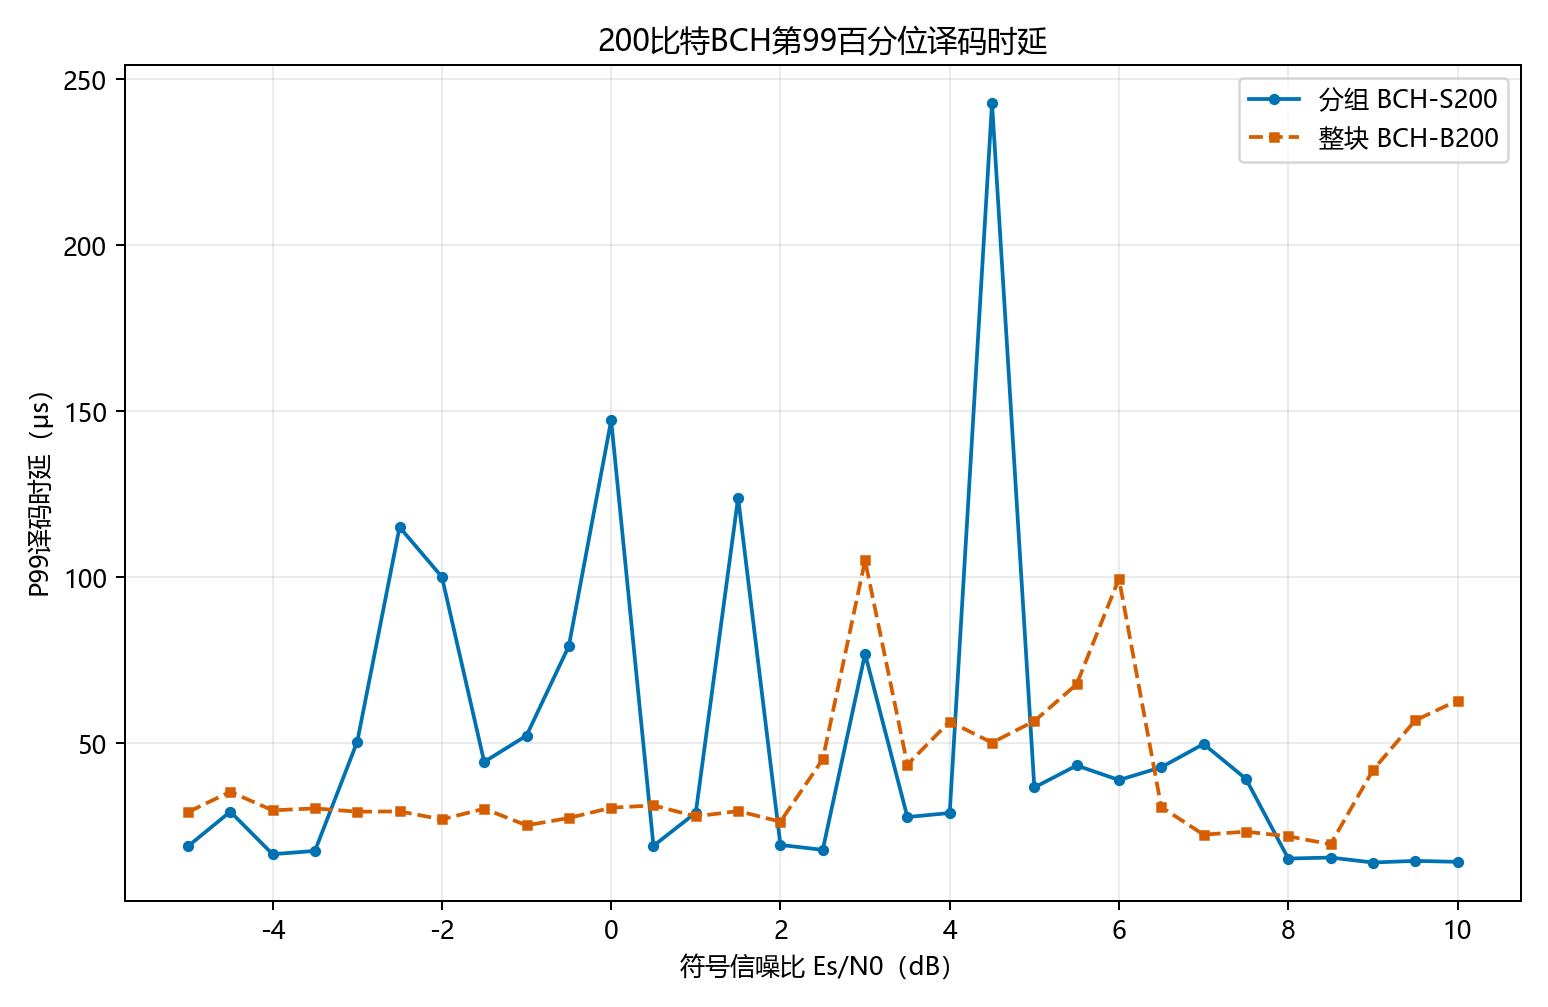
\includegraphics[width=0.98\linewidth]{../Task/Comparison/S6/results/summary/figures/bch_09_p99_time/figure.png}\\[-0.2em]\small（c）P99时间
  \end{minipage}\hfill
  \begin{minipage}{0.49\textwidth}\centering
    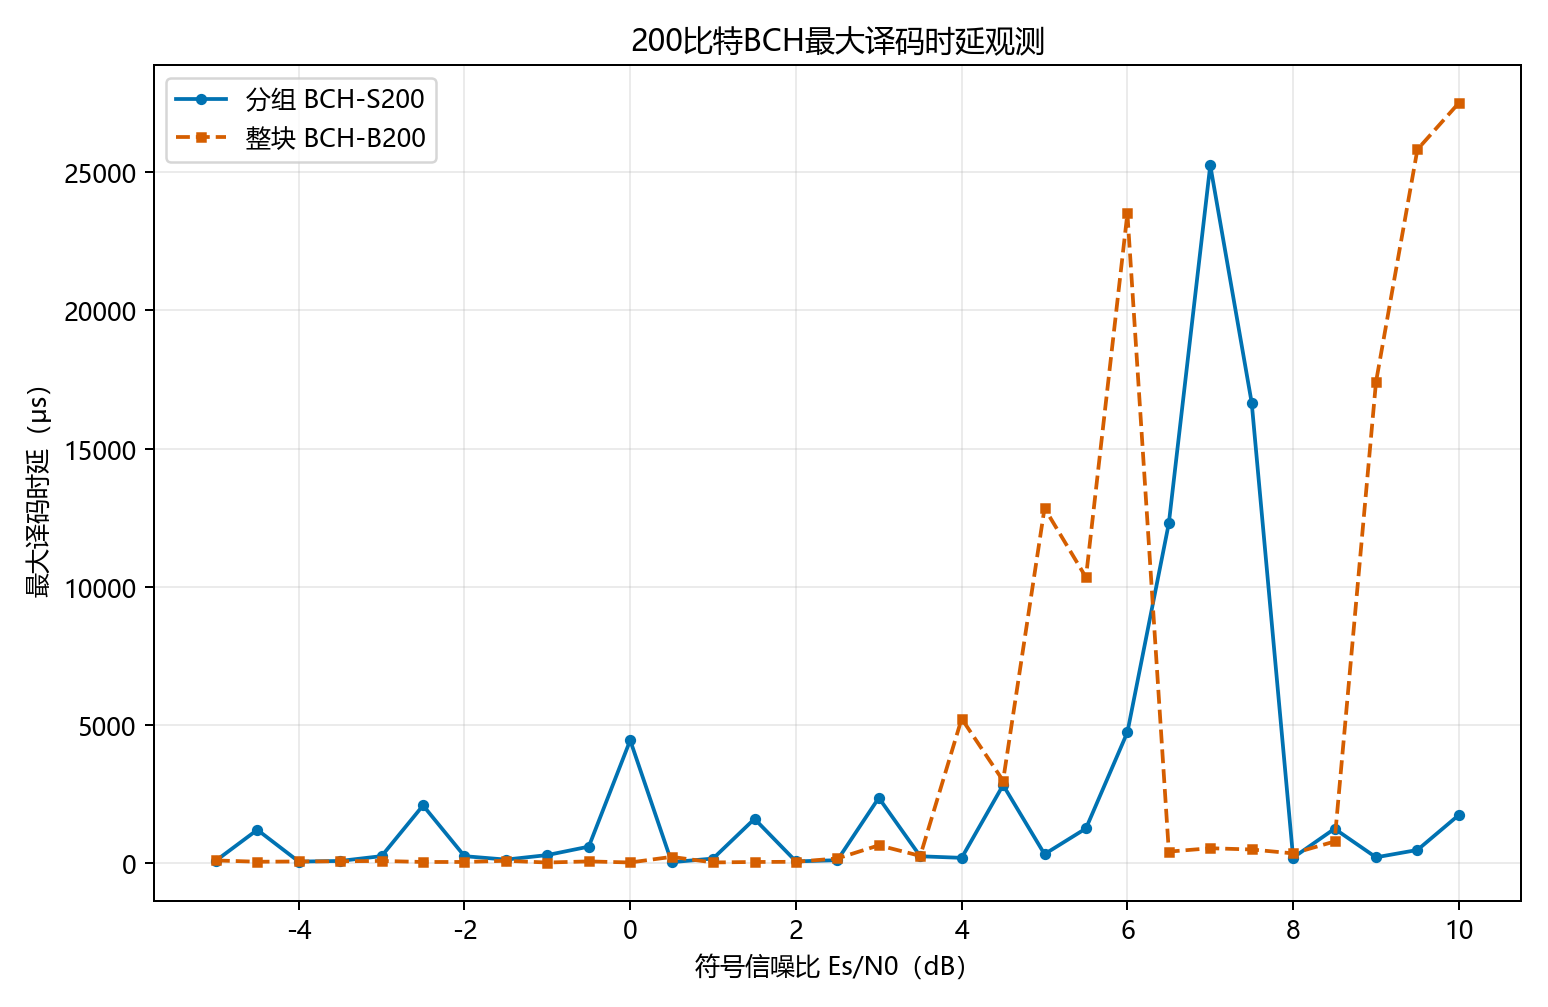
\includegraphics[width=0.98\linewidth]{../Task/Comparison/S6/results/summary/figures/bch_10_max_time/figure.png}\\[-0.2em]\small（d）最大观测时间
  \end{minipage}
  \caption{BCH译码时间统计}
  \label{fig:s6-bch-time}
\end{figure}

\begin{table}[htbp]
  \centering
  \scriptsize
  \caption{BCH可靠性、资源与软件时间汇总}
  \label{tab:s6-bch-summary}
  \setlength{\tabcolsep}{2.1pt}
  \begin{tabular}{p{0.12\textwidth}ccccc p{0.20\textwidth}}
    \toprule
    方案 & FER=0.1/dB & FER=0.01/dB & 加权平均/$\mu$s & 最大观测/$\mu$s & 内存/byte & 主要计算结构 \\
    \midrule
    BCH-S200 & 4.667 & 6.040 & 10.217 & 25240.3 & 1580 & 19组综合征、查表、翻转和译后检查 \\
    BCH-B200 & 3.612 & 4.369 & 17.415 & 27491.4 & 2408 & 综合征、BM、Chien及有限域运算 \\
    \bottomrule
  \end{tabular}
\end{table}

\subsection{BCH工程结论}

在本项目既定实现中，BCH-S200的短分组、固定查表和较小工作区形成了更低的软件时间与更简单的实现结构，适合资源受限且允许较高链路信噪比的场景。BCH-B200以BM、Chien搜索和有限域表开销换取整块$t=6$纠错能力，在FER为0.01时比S200节省1.671 dB，同时平均软件译码时间增加约70.5\%、模型内存增加52.4\%。该权衡属于完整编码组织和译码结构共同变化的结果，不应归因于单一译码算法。

\section{卷积码硬判决与软判决Viterbi对比}

\subsection{正式配置与判决定义}

卷积码使用300 bit载荷和6个终止比特，$R=1/2$不打孔，实际发送612 bit，实际码率为0.4902。整块方案一次处理306个网格输入步，$D=W=306$、$S=300$；连续方案按50$\times$6、100$\times$3和150$\times$2三种业务组织输入，均使用回溯深度$D=70$、窗口长度$W=128$和滑动步长$S=25$。硬判决把接收样值阈值化为0/1比特，以汉明距离构造分支度量；浮点软判决保留连续BPSK接收符号，以接收符号与理想$\pm1$符号之间的欧氏距离平方构造分支度量，并非LLR输入。

卷积码证据复用S3 Stage14的正式仿真数据并在S6中统一整理，S6没有按相同停止时刻重新执行逐帧strict pair-stop。因此，本节依据相同配置、信噪比网格和正式统计曲线比较硬、软判决差异，不进行逐帧差分因果推断。该限制不否定已有统计结果，但限定了结论的精度和表达范围。

\subsection{BER、FER与门限差异}

图\ref{fig:s6-cc-reliability}显示，整块和三种连续组织下，浮点软判决均比硬判决更早进入低错误率区。整块方案在FER为0.1时，软、硬判决门限分别为$-0.731$ dB和1.367 dB，软判决节省2.098 dB；在FER为0.01时，两者分别为0.229 dB和2.489 dB，差值为2.260 dB。三种连续组织的FER曲线及门限与整块统计一致，说明在当前终止、窗口和输出组织下，可靠性差异主要由判决信息精度决定，而组织方式主要改变执行与输出时序。

\begin{figure}[p]
  \centering
  \begin{minipage}{0.92\textwidth}\centering
    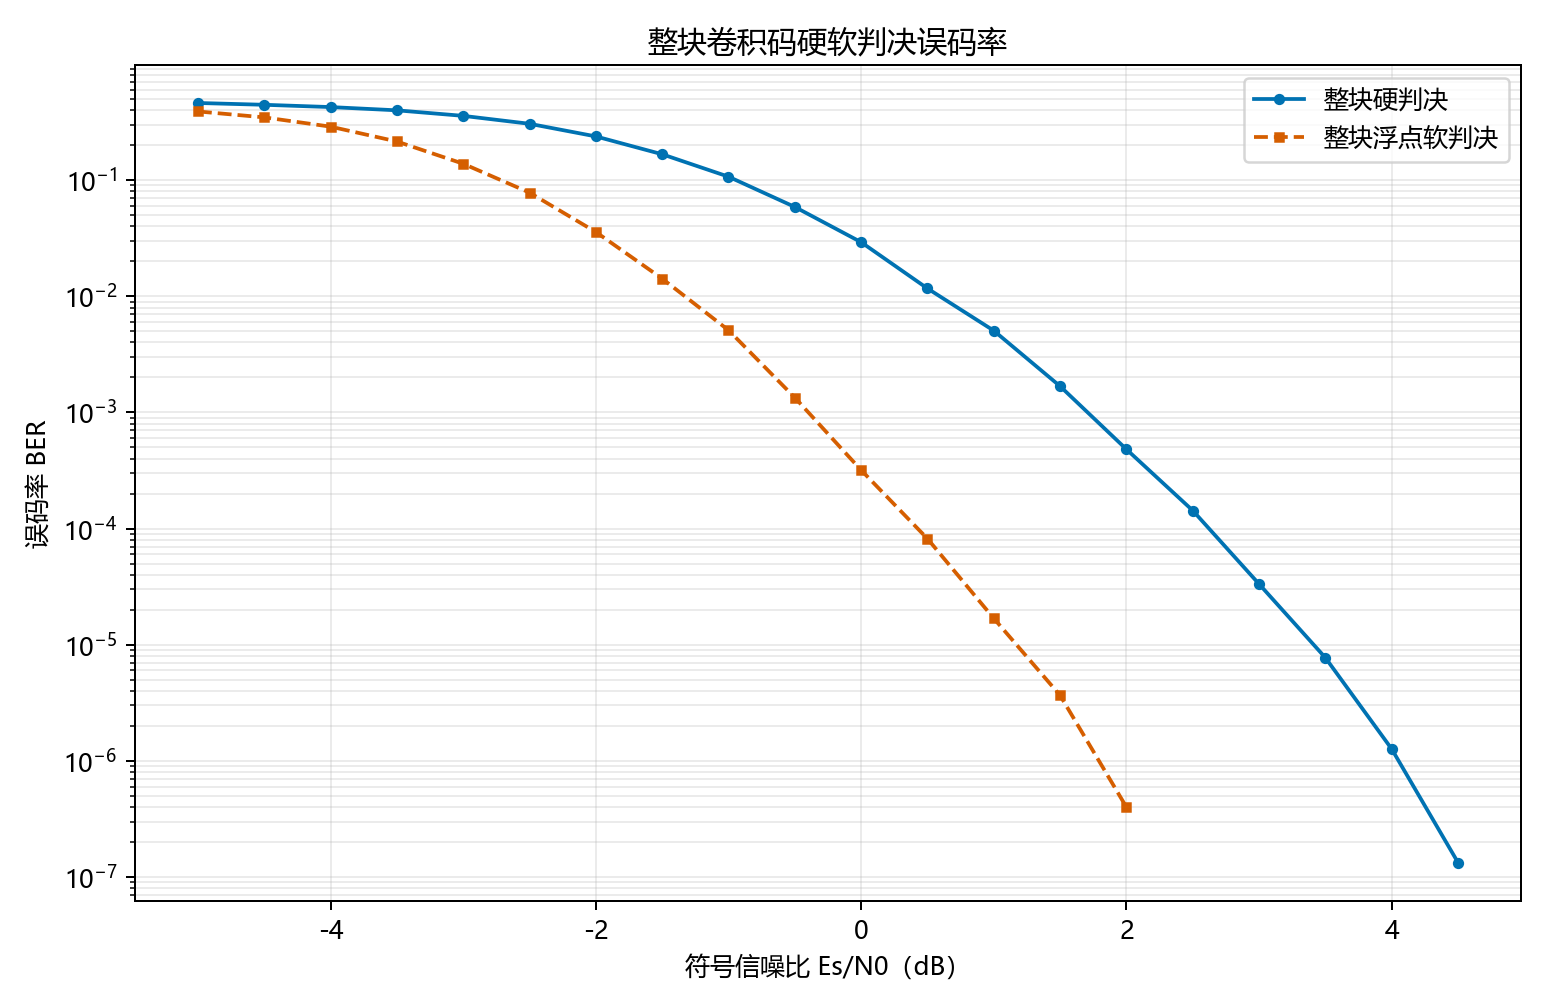
\includegraphics[width=0.70\linewidth]{../Task/Comparison/S6/results/summary/figures/cc_01_block_ber/figure.png}\\[-0.2em]\small（a）整块译码BER
  \end{minipage}\par\medskip
  \begin{minipage}{0.92\textwidth}\centering
    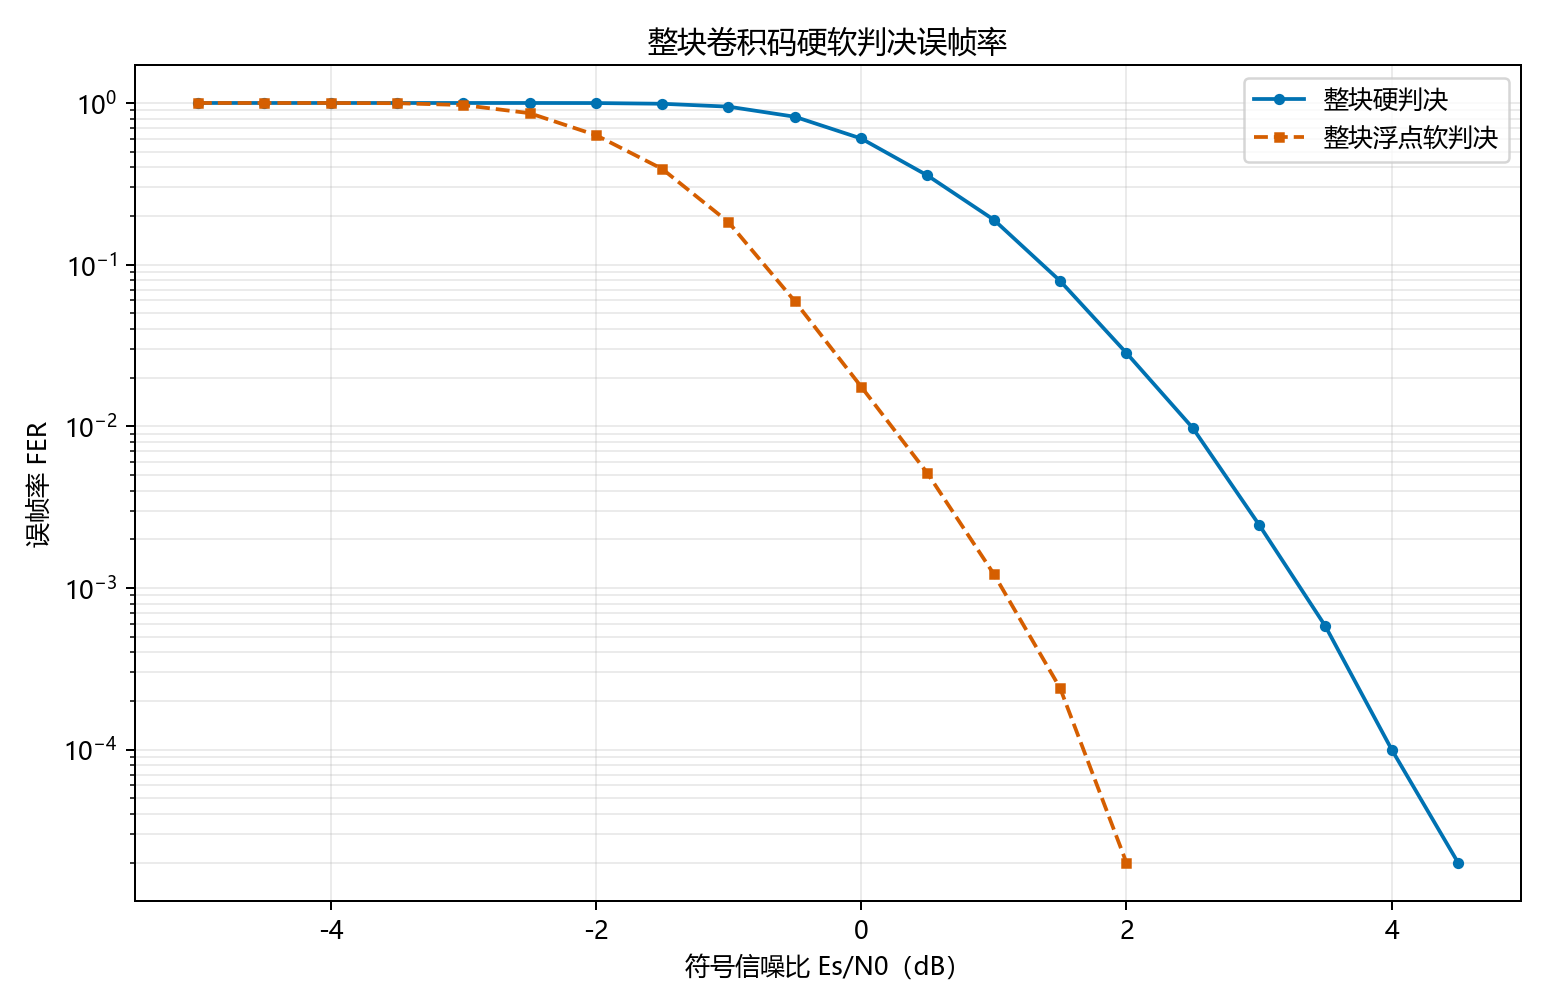
\includegraphics[width=0.70\linewidth]{../Task/Comparison/S6/results/summary/figures/cc_02_block_fer/figure.png}\\[-0.2em]\small（b）整块译码FER
  \end{minipage}\par\medskip
  \begin{minipage}{0.92\textwidth}\centering
    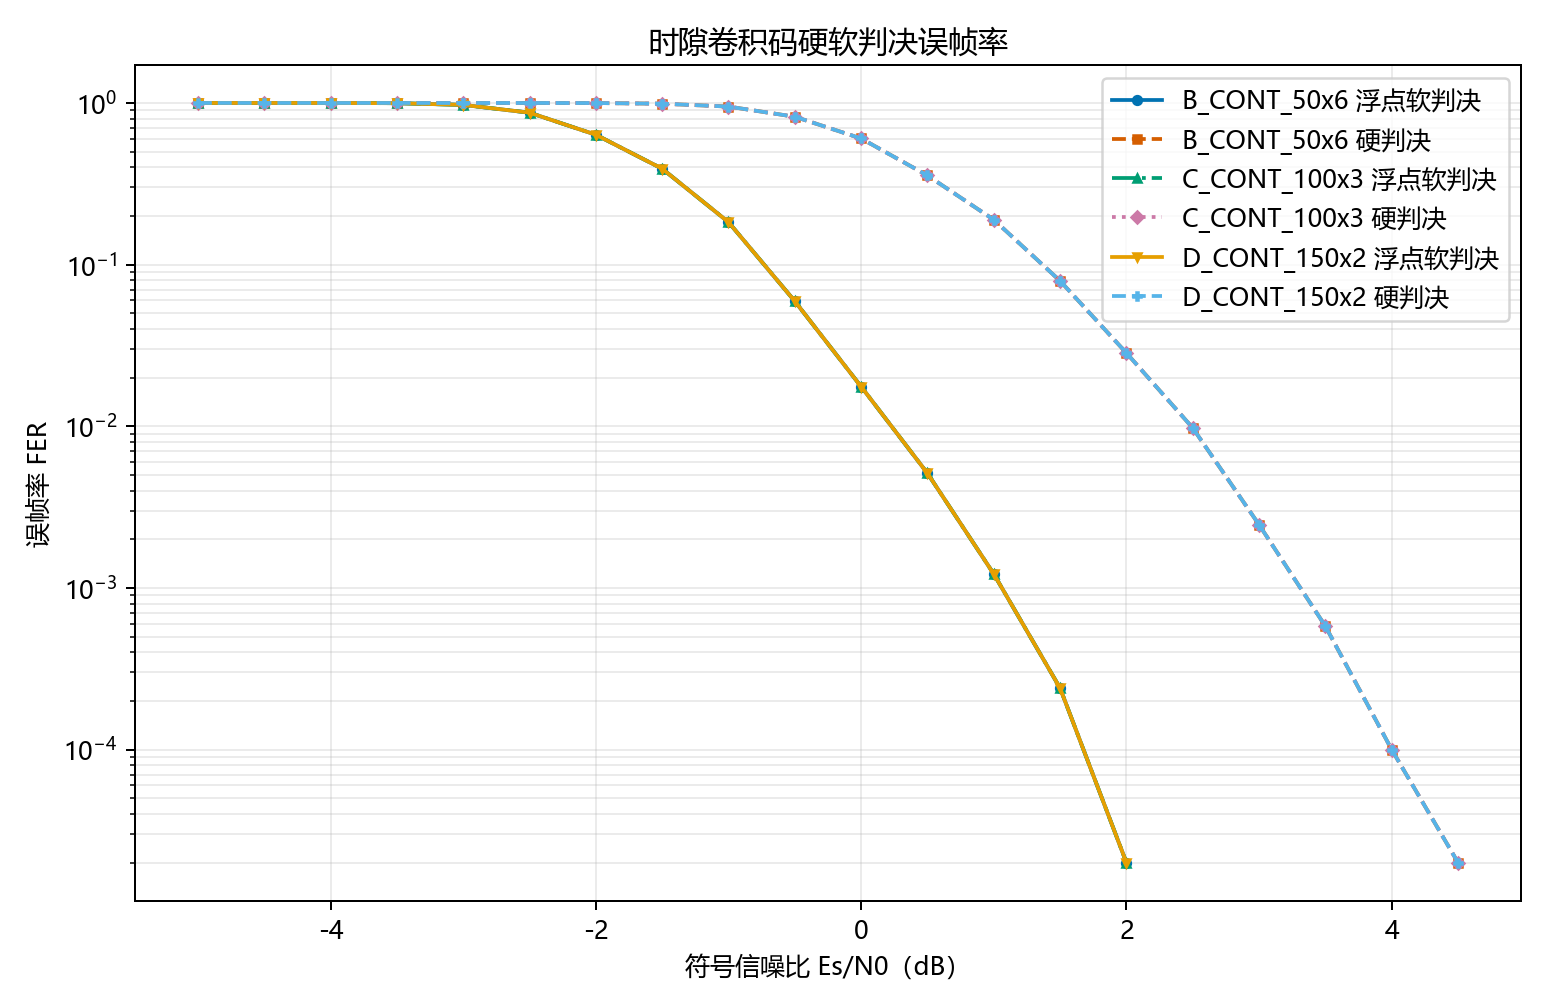
\includegraphics[width=0.70\linewidth]{../Task/Comparison/S6/results/summary/figures/cc_03_slot_fer/figure.png}\\[-0.2em]\small（c）连续组织FER
  \end{minipage}
  \caption{卷积码硬判决与浮点软判决的BER和FER}
  \label{fig:s6-cc-reliability}
\end{figure}

\begin{table}[htbp]
  \centering
  \scriptsize
  \caption{卷积码硬判决与浮点软判决的可靠性门限}
  \label{tab:s6-cc-thresholds}
  \setlength{\tabcolsep}{2.4pt}
  \begin{tabular}{p{0.16\textwidth}p{0.12\textwidth}ccc p{0.18\textwidth}}
    \toprule
    组织方式 & 判决 & FER=0.1/dB & FER=0.01/dB & 相对硬判决增益/dB & 说明 \\
    \midrule
    整块及三种连续组织 & 硬判决 & 1.367 & 2.489 & 0 & 1 bit判决，汉明距离分支度量 \\
    整块及三种连续组织 & 浮点软判决 & $-0.731$ & 0.229 & 2.098/2.260 & 连续符号，欧氏距离平方分支度量 \\
    \bottomrule
  \end{tabular}
\end{table}

\subsection{复杂度、存储与软件时间}

硬、软Viterbi采用相同状态数、候选分支数、ACS骨架和回溯骨架，因此图\ref{fig:s6-cc-resource}中同一组织的ACS与回溯计数相同。整块译码每帧39168次ACS和306次回溯操作；连续组织因窗口重复处理，每帧约143998次ACS和866次回溯操作。相同ACS计数不表示总计算代价相同：硬判决分支度量以比特比较和汉明距离为主，浮点软判决需要减法、平方和加法。模型内存由组织方式决定，整块为59776 byte，连续窗口为26112 byte，判决精度在当前内存模型中没有改变这一数值。

\begin{figure}[p]
  \centering
  \begin{minipage}{0.92\textwidth}\centering
    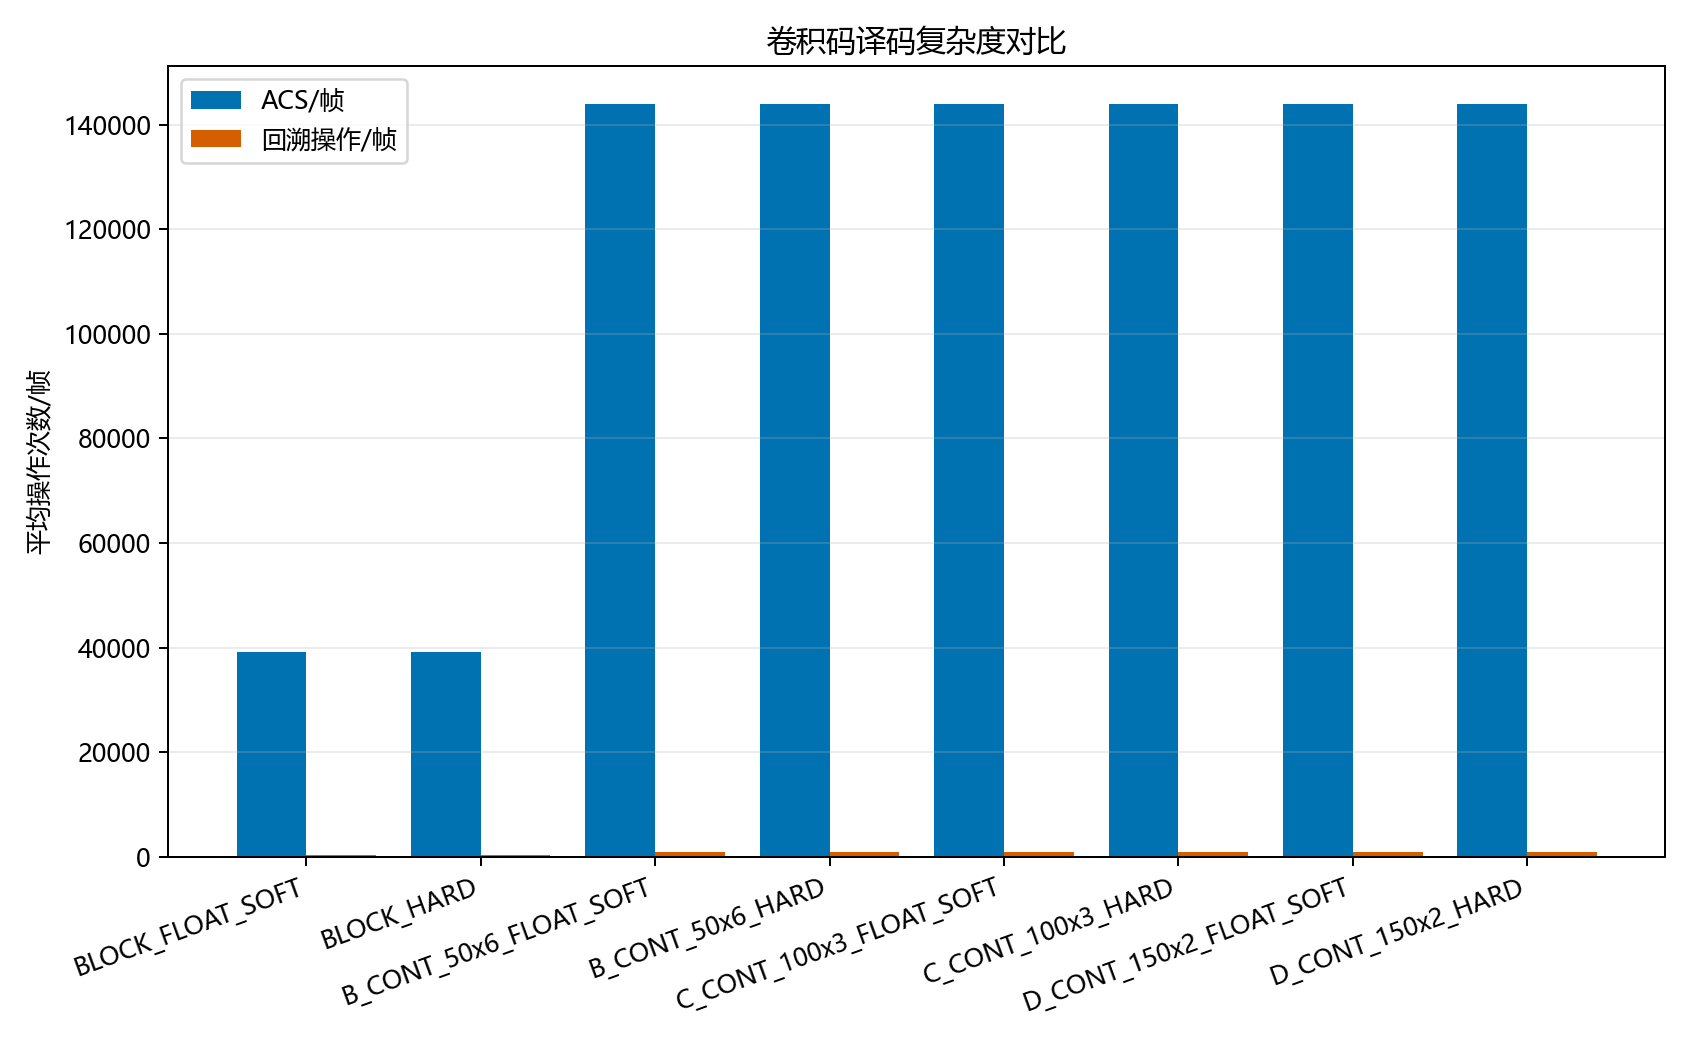
\includegraphics[width=0.90\linewidth]{../Task/Comparison/S6/results/summary/figures/cc_04_complexity/figure.png}\\[-0.2em]\small（a）ACS与回溯操作
  \end{minipage}\par\medskip
  \begin{minipage}{0.92\textwidth}\centering
    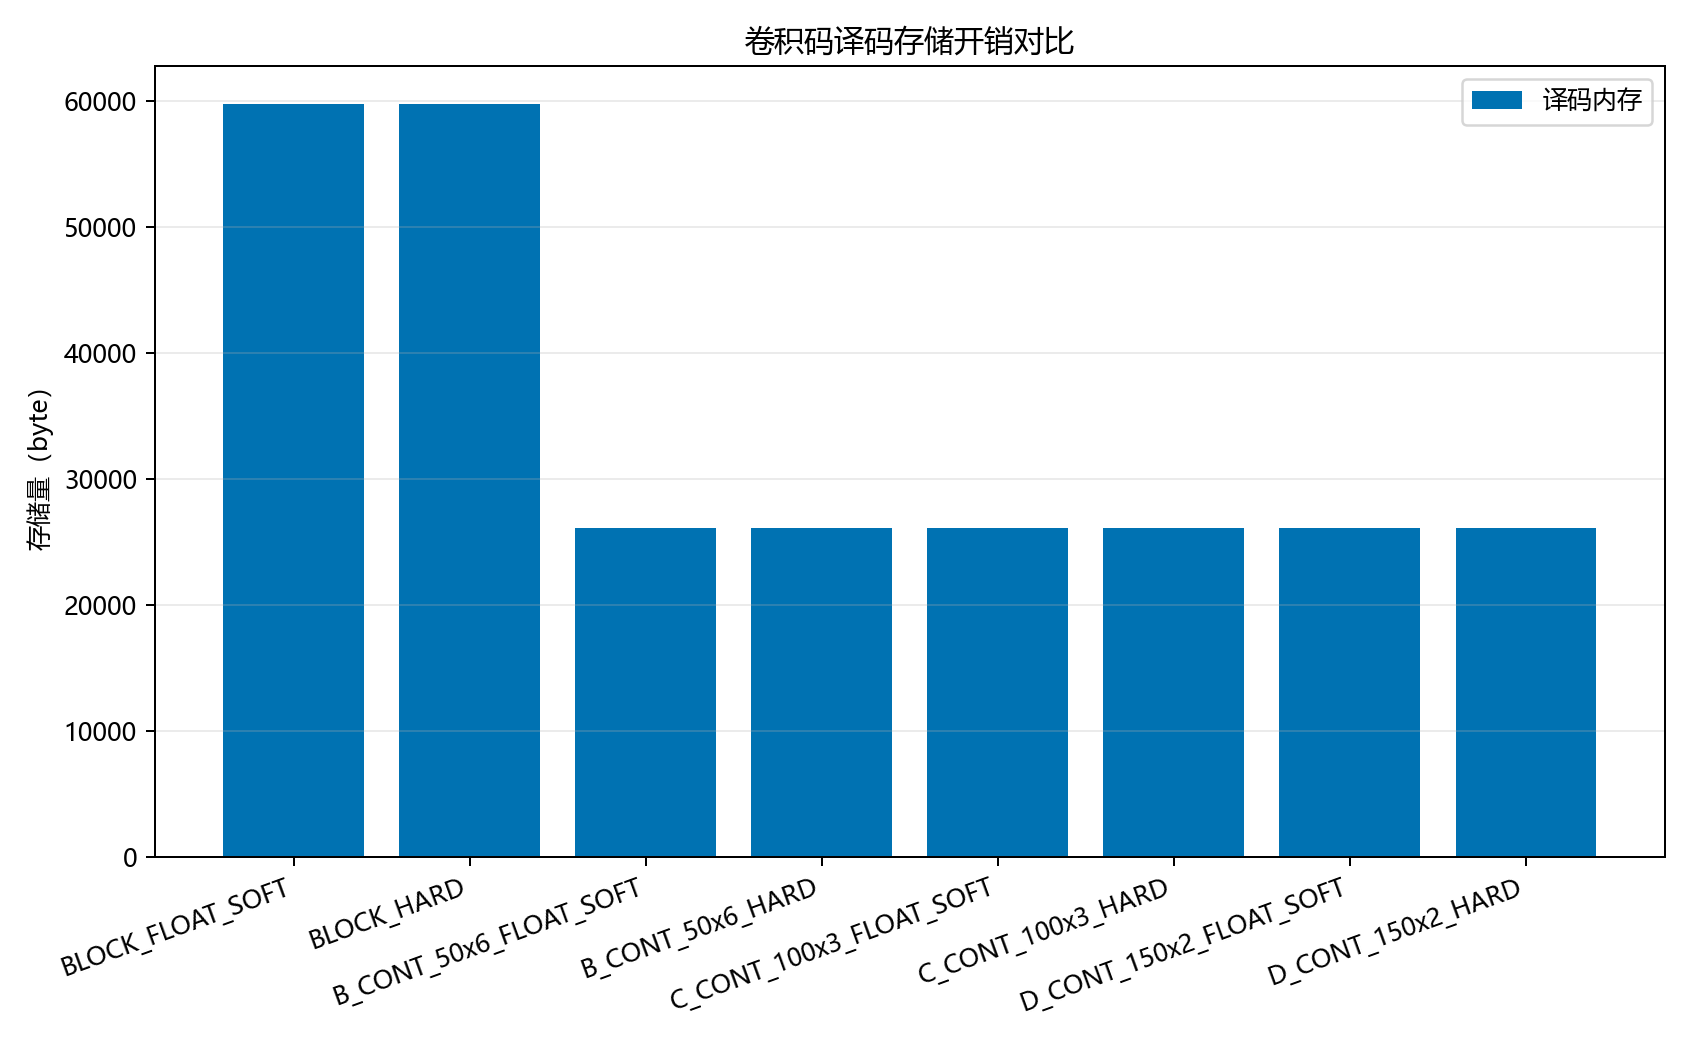
\includegraphics[width=0.90\linewidth]{../Task/Comparison/S6/results/summary/figures/cc_05_memory/figure.png}\\[-0.2em]\small（b）译码器内存
  \end{minipage}
  \caption{卷积码Viterbi译码的操作规模与存储开销}
  \label{fig:s6-cc-resource}
\end{figure}

图\ref{fig:s6-cc-latency}区分CPU软件译码时间、首输出时延和决策时延。整块硬、软判决的帧加权平均译码时间分别为339.03~$\mu$s和524.00~$\mu$s，浮点软判决增加54.6\%；最大观测时间分别为34231.5~$\mu$s和65607.2~$\mu$s。三种连续组织的硬判决加权平均时间为1549.17--1565.58~$\mu$s，软判决为1835.82--1849.69~$\mu$s，增加约18\%。连续组织的首输出时延为298或398个符号，平均决策时延图所示值为342、430或530个符号；二者由到达批次、窗口和回溯调度决定，不能称为平均译码时间或最大译码时间。

\begin{figure}[p]
  \centering
  \begin{minipage}{0.92\textwidth}\centering
    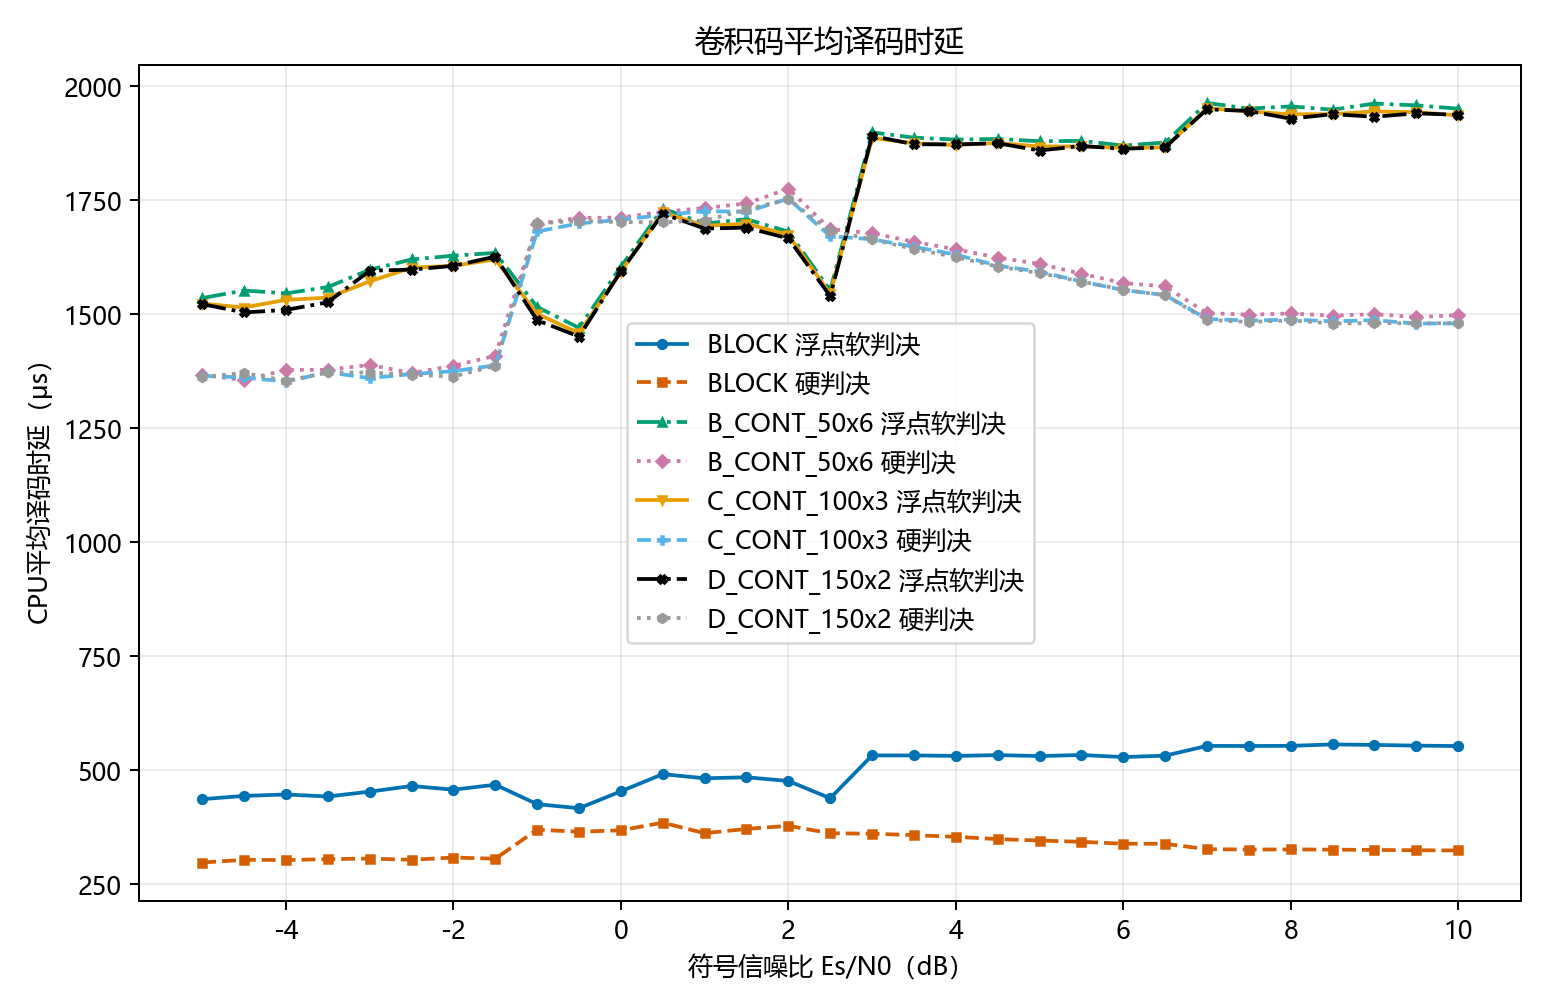
\includegraphics[width=0.90\linewidth]{../Task/Comparison/S6/results/summary/figures/cc_06_avg_time/figure.png}\\[-0.2em]\small（a）平均CPU译码时间
  \end{minipage}\par\medskip
  \begin{minipage}{0.49\textwidth}\centering
    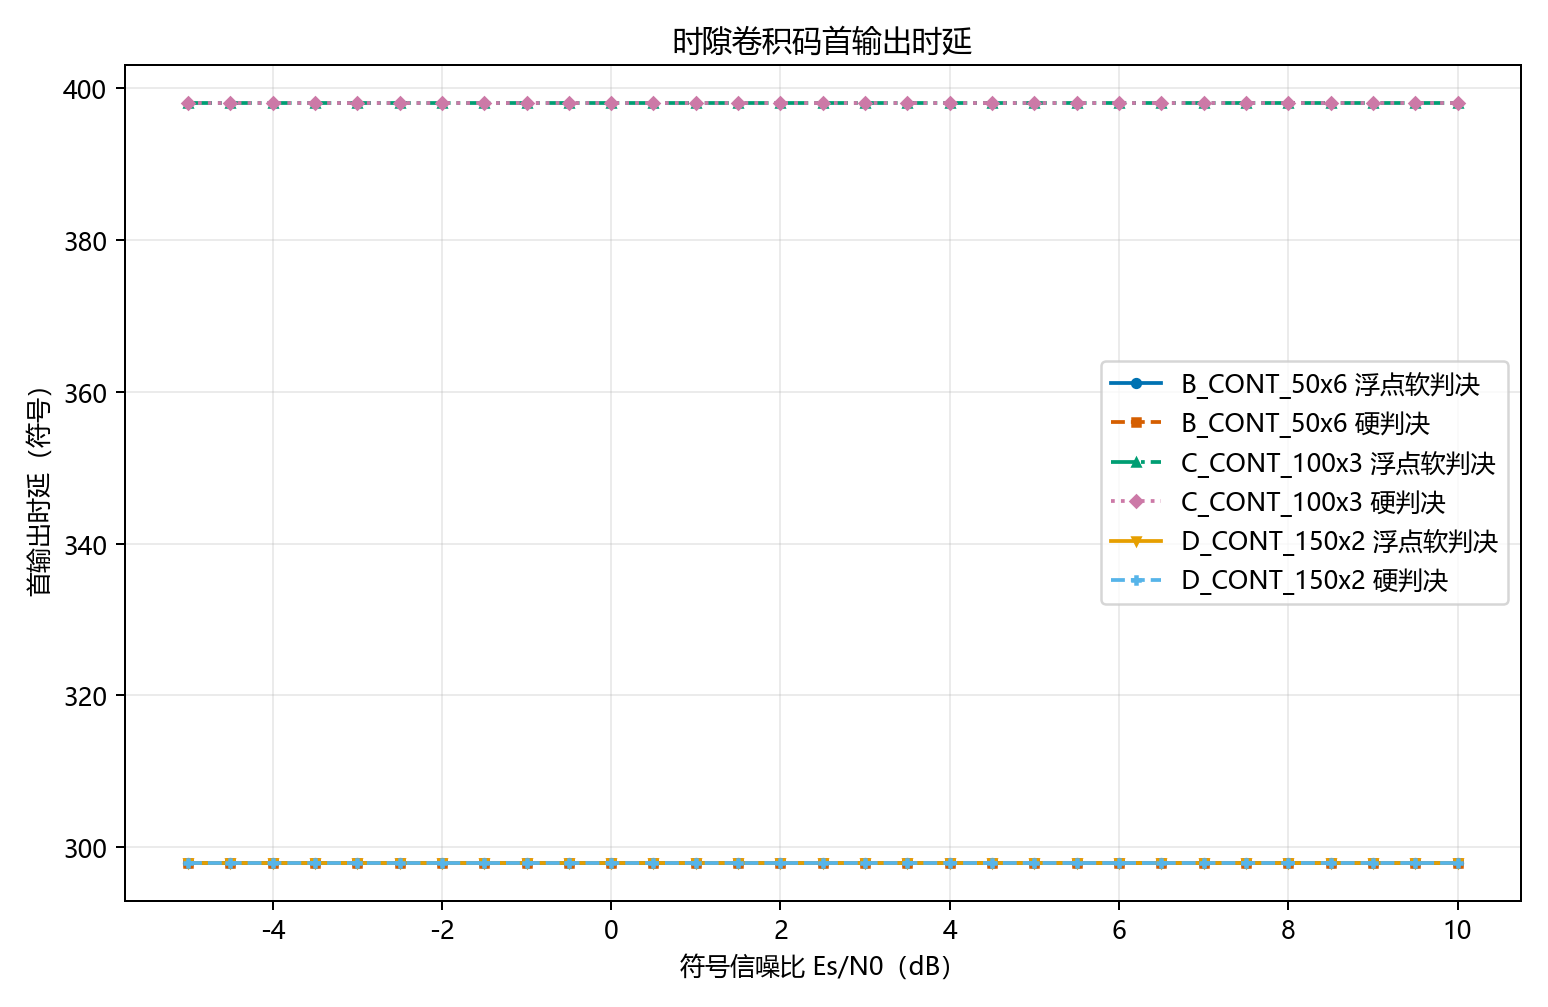
\includegraphics[width=0.98\linewidth]{../Task/Comparison/S6/results/summary/figures/cc_07_first_output/figure.png}\\[-0.2em]\small（b）首输出时延
  \end{minipage}\hfill
  \begin{minipage}{0.49\textwidth}\centering
    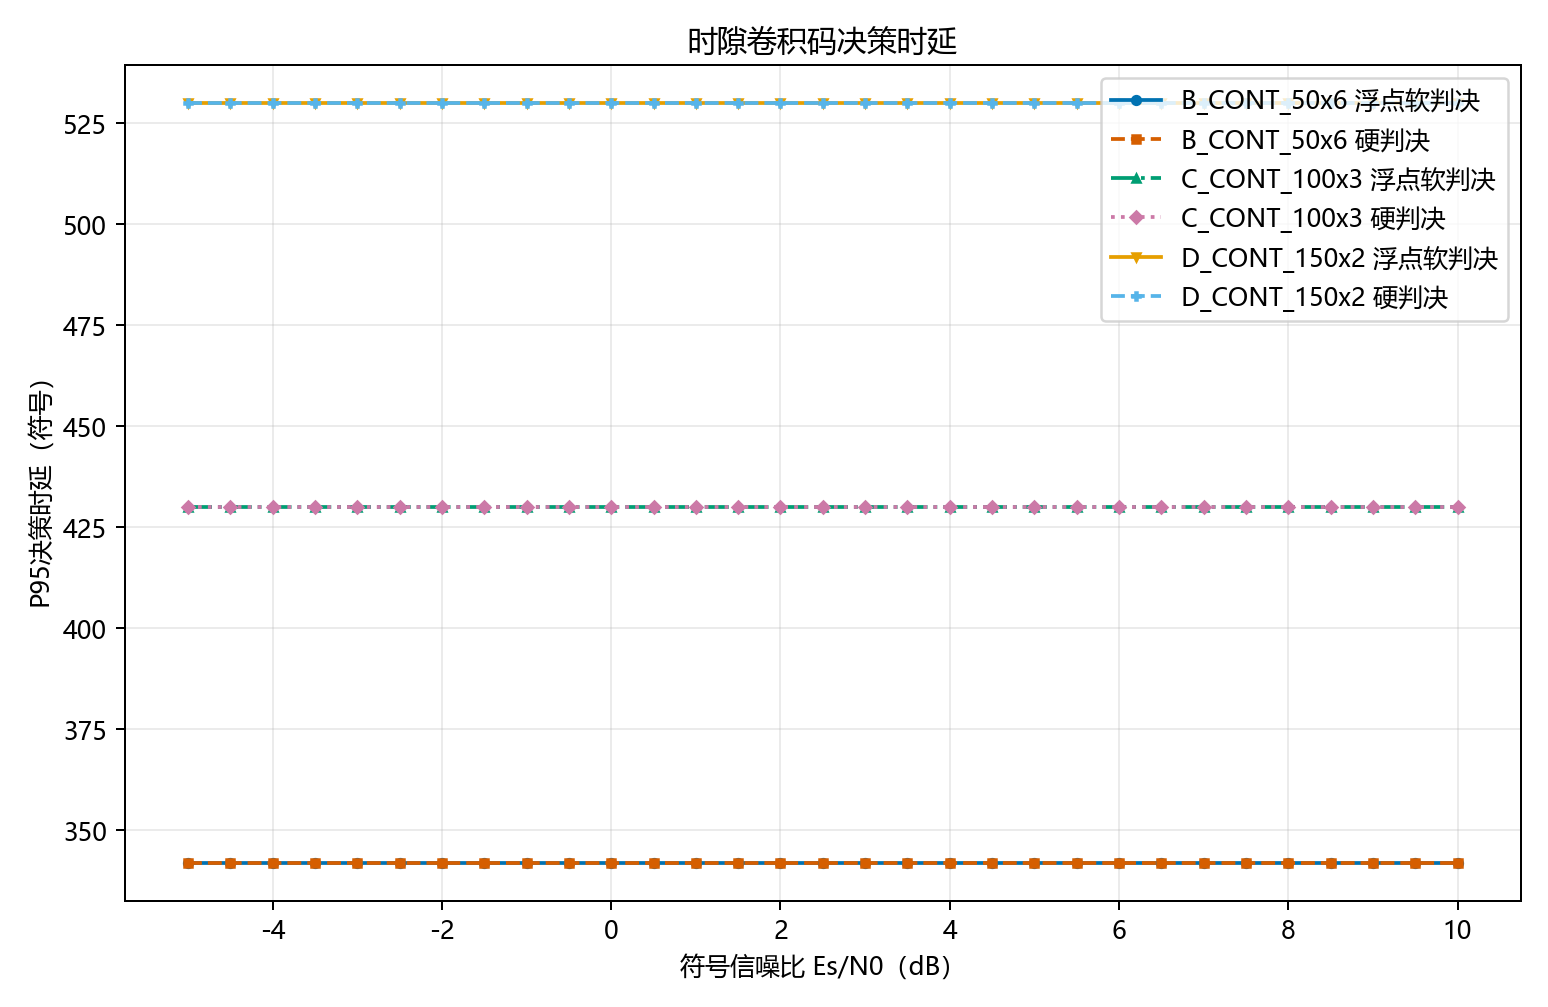
\includegraphics[width=0.98\linewidth]{../Task/Comparison/S6/results/summary/figures/cc_08_decision_delay/figure.png}\\[-0.2em]\small（c）决策时延
  \end{minipage}
  \caption{卷积码Viterbi译码的软件时间与流式输出时延}
  \label{fig:s6-cc-latency}
\end{figure}

\begin{table}[htbp]
  \centering
  \scriptsize
  \caption{硬判决与浮点软判决Viterbi的计算结构和实现代价}
  \label{tab:s6-cc-cost}
  \setlength{\tabcolsep}{2.0pt}
  \begin{tabular}{p{0.11\textwidth}p{0.18\textwidth}p{0.17\textwidth}p{0.14\textwidth}p{0.13\textwidth}p{0.17\textwidth}}
    \toprule
    判决 & 分支度量 & 共同骨架 & 整块加权平均/$\mu$s & 整块最大/$\mu$s & 工程特征 \\
    \midrule
    硬判决 & 0/1比特与汉明距离 & 相同状态、候选分支、ACS和回溯 & 339.03 & 34231.5 & 计算精度要求低，可靠性损失较大 \\
    浮点软判决 & 连续符号与欧氏距离平方 & 相同状态、候选分支、ACS和回溯 & 524.00 & 65607.2 & 保留幅值可靠性信息，分支度量更重 \\
    \bottomrule
  \end{tabular}
\end{table}

\subsection{卷积码工程结论}

浮点软判决以更重的分支度量换取约2.10--2.26 dB的FER门限收益，适合链路可靠性优先、具备浮点或等效定点度量资源的接收机。硬判决降低输入精度和分支度量实现要求，适合资源或实时性更受约束且链路余量足够的场景。连续窗口方案减小模型内存并提供分批输出，但窗口重复计算使当前串行软件时间高于整块方案；首输出与决策时延应作为独立流式指标使用。

\section{LDPC BP与NMS译码对比}

\subsection{正式配置与配对条件}

S6采用BG2 Direct QC-LDPC的N560实例。老师给出的名义目标长度为576 bit，Direct BG2候选选择器最终映射到实际长度560 bit，因此本章与图表均称为N560。载荷为300 bit，实际码率为$300/560=0.5357$，提升因子$Z_c=56$，信息容量448 bit，填充148 bit，校验长度112 bit，校验子矩阵秩为112。BP与NMS的最大迭代次数均为32，均在完成一次完整迭代后计算综合征并提前停止，NMS归一化系数为$\alpha=0.95$。

\begin{table}[htbp]
  \centering
  \scriptsize
  \caption{S6 LDPC译码算法比较配置}
  \label{tab:s6-ldpc-config}
  \setlength{\tabcolsep}{2.4pt}
  \begin{tabular}{p{0.17\textwidth}p{0.20\textwidth}p{0.17\textwidth}p{0.20\textwidth}p{0.16\textwidth}}
    \toprule
    项目 & 数值 & 项目 & 数值 & 说明 \\
    \midrule
    实际案例 & N560 & 载荷/码长 & 300/560 bit & 名义目标576映射到实际560 \\
    实际码率 & 0.5357 & $Z_c$ & 56 & BG2 Direct QC-LDPC \\
    填充/校验 & 148/112 bit & $\mathrm{rank}(H_p)$ & 112 & 不使用速率匹配与交织 \\
    译码器 & 分层BP、分层NMS & 最大迭代 & 32 & 完整迭代后综合征提前停止 \\
    NMS系数 & $\alpha=0.95$ & 配对输入 & 载荷、码字、LLR & 31个信噪比点哈希一致 \\
    \bottomrule
  \end{tabular}
\end{table}

BP和NMS共享同一载荷、码字、噪声、对数似然比（Log-Likelihood Ratio，LLR）、校验图、最大迭代次数和提前停止规则，只改变校验节点消息更新。逐信噪比的载荷、码字和LLR哈希均一致，使该对比能够把可靠性与时间差异较严格地归因于校验节点更新结构。

\subsection{BER与FER}

图\ref{fig:s6-ldpc-reliability}中BP与NMS曲线在瀑布区基本重合，NMS表现出轻微性能损失。FER为0.1时，BP和NMS所需$E_s/N_0$分别为4.541 dB和4.577 dB，NMS损失0.036 dB；FER为0.01时，两者分别为5.866 dB和5.875 dB，损失0.010 dB。两种算法各有4个零BER/FER工作点，零值没有用于门限外推。当前$\alpha=0.95$配置因此在两个目标FER处保留了接近BP的可靠性。

\begin{figure}[p]
  \centering
  \begin{minipage}{0.92\textwidth}\centering
    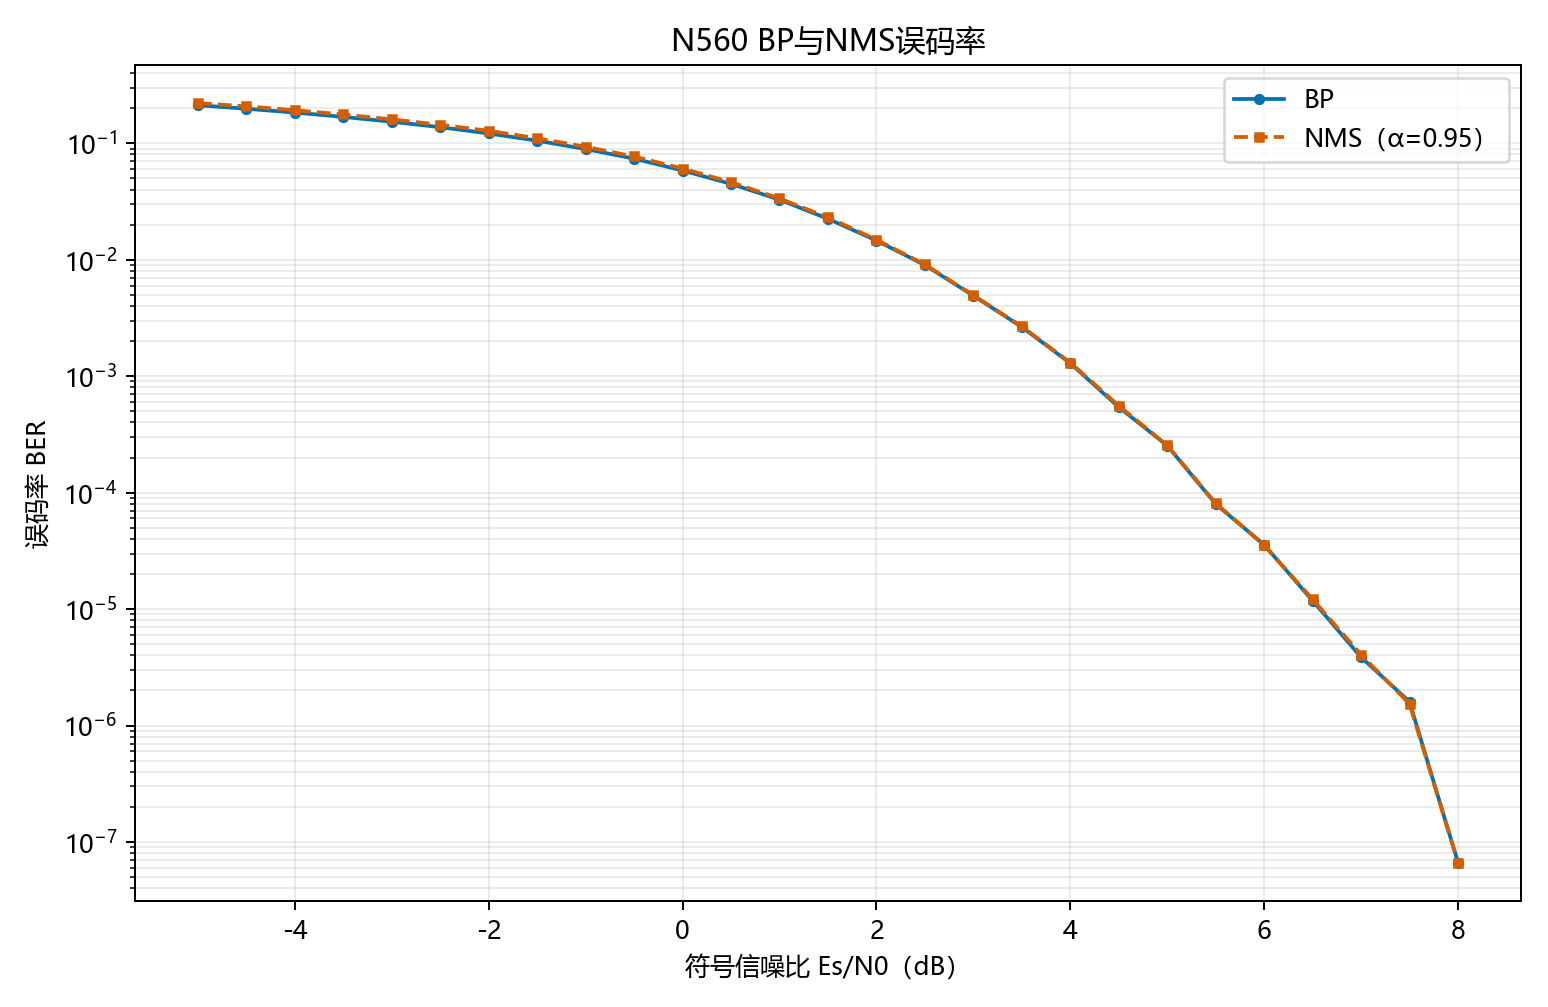
\includegraphics[width=0.90\linewidth]{../Task/Comparison/S6/results/summary/figures/ldpc_01_ber/figure.png}\\[-0.2em]\small（a）比特错误率
  \end{minipage}\par\medskip
  \begin{minipage}{0.92\textwidth}\centering
    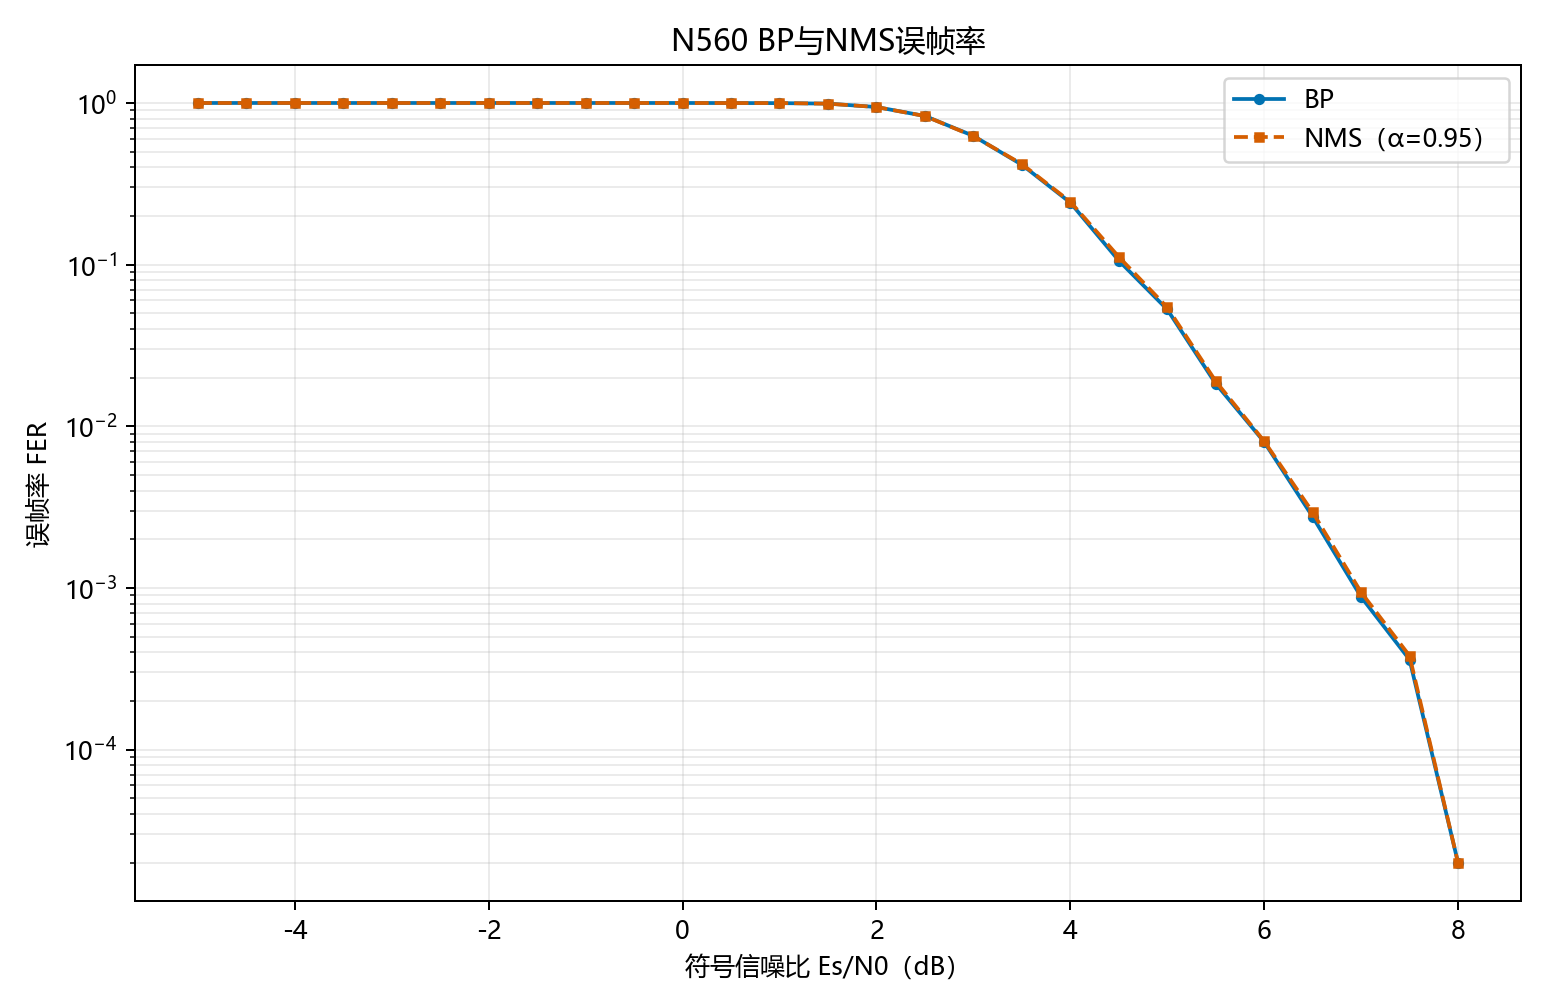
\includegraphics[width=0.90\linewidth]{../Task/Comparison/S6/results/summary/figures/ldpc_02_fer/figure.png}\\[-0.2em]\small（b）帧错误率
  \end{minipage}
  \caption{LDPC BP与NMS译码的BER和FER}
  \label{fig:s6-ldpc-reliability}
\end{figure}

\subsection{迭代与提前停止行为}

图\ref{fig:s6-ldpc-convergence}表明，低信噪比区的大量帧达到32次上限，进入瀑布区后平均迭代数随可靠性提高而下降，提前停止率相应上升。31点等权网格均值中，BP和NMS平均迭代数分别为16.44和13.11；其逐点范围分别为1--32次和1--28.47次。NMS在部分低信噪比点出现较高提前停止率，其中可能包含错误码字满足校验的情况，不能把“提前停止”单独解释为可靠译码成功。总软件代价同时取决于迭代次数和单次迭代计算结构，不能只用平均迭代数判断复杂度。

\begin{figure}[p]
  \centering
  \begin{minipage}{0.92\textwidth}\centering
    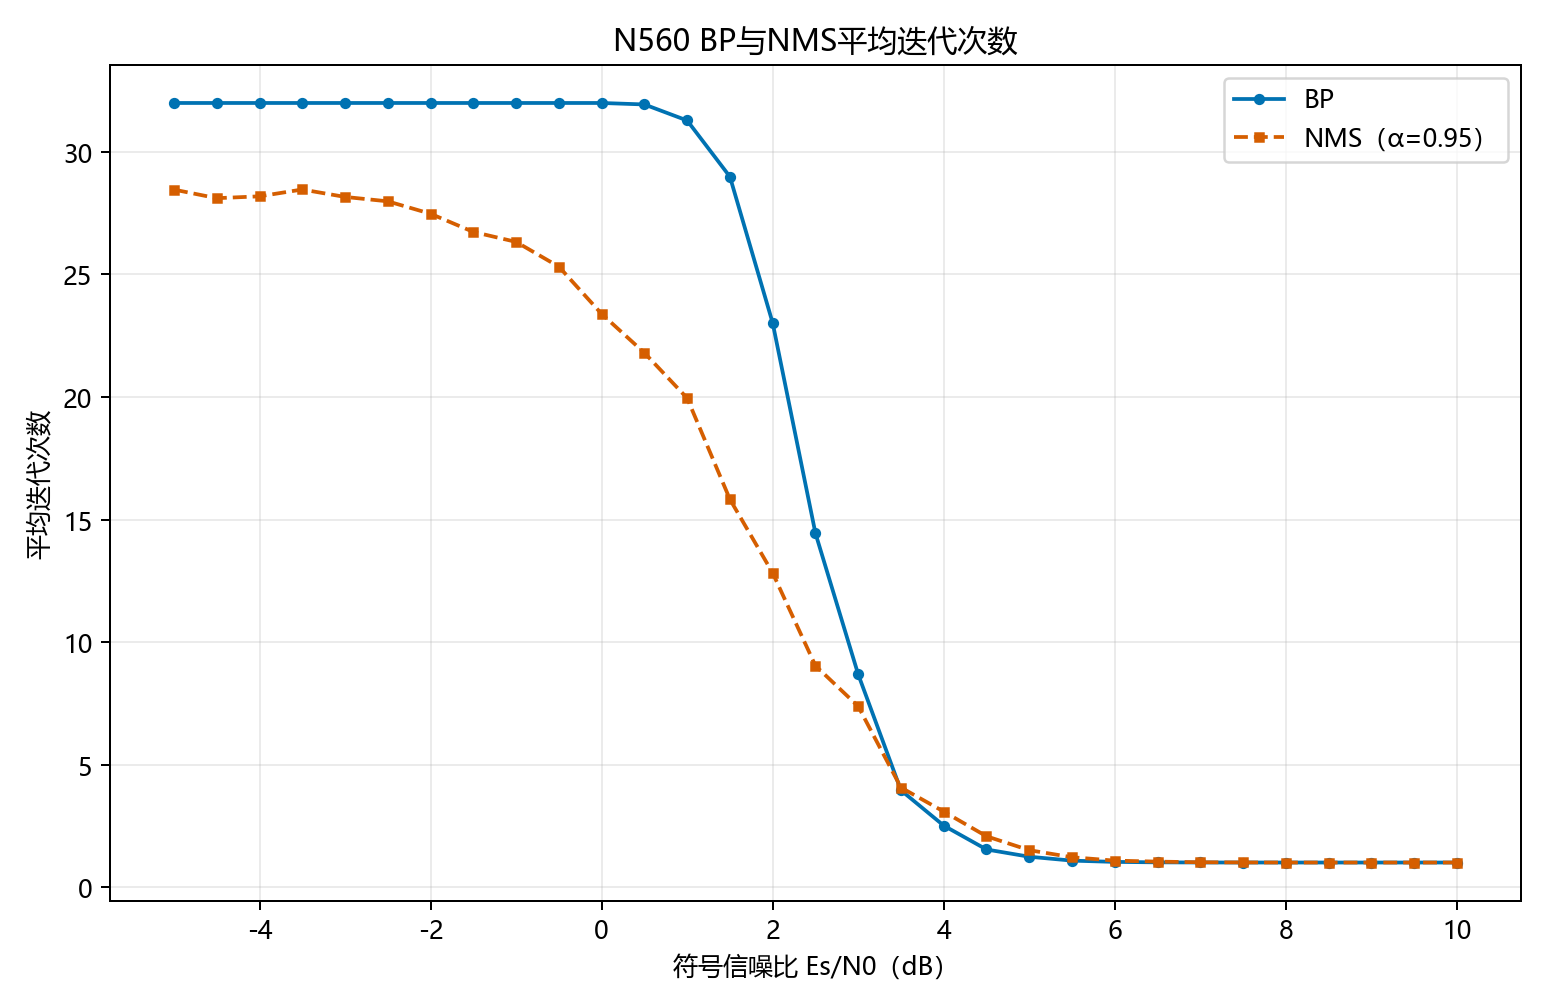
\includegraphics[width=0.90\linewidth]{../Task/Comparison/S6/results/summary/figures/ldpc_03_iterations/figure.png}\\[-0.2em]\small（a）平均迭代次数
  \end{minipage}\par\medskip
  \begin{minipage}{0.92\textwidth}\centering
    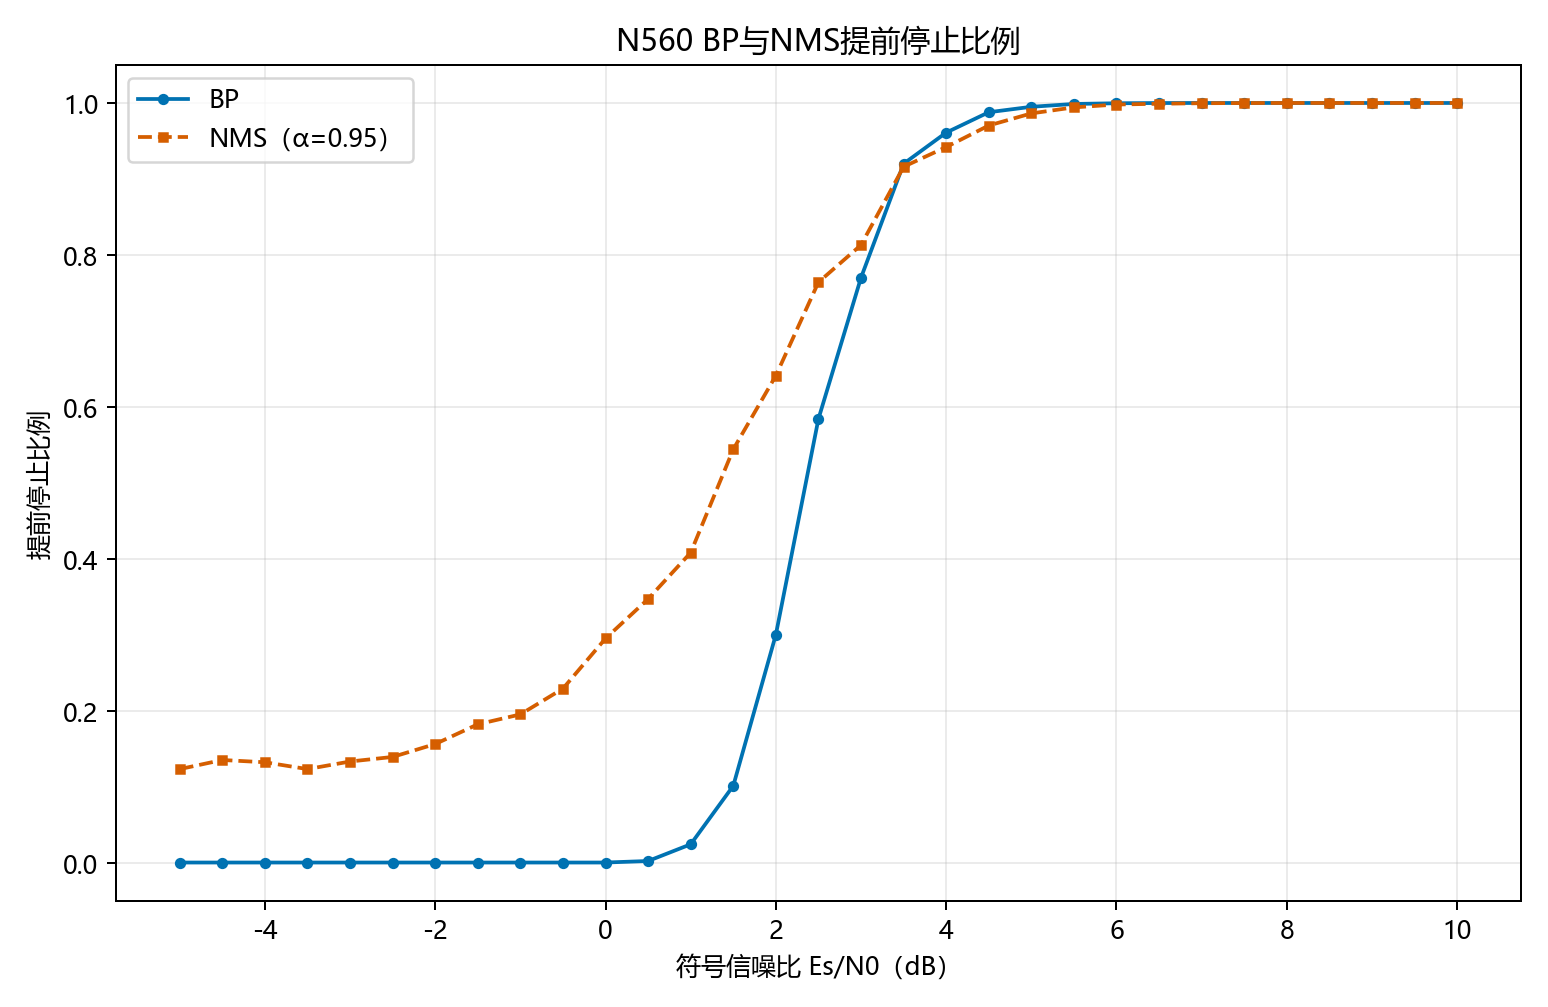
\includegraphics[width=0.90\linewidth]{../Task/Comparison/S6/results/summary/figures/ldpc_04_early_stop/figure.png}\\[-0.2em]\small（b）提前停止率
  \end{minipage}
  \caption{LDPC BP与NMS的迭代和提前停止行为}
  \label{fig:s6-ldpc-convergence}
\end{figure}

\subsection{复杂度、存储与软件译码时间}

BP校验节点更新包含双曲正切、反双曲正切及消息更新；NMS以绝对值、符号、第一/第二最小值、比较和$\alpha$缩放近似非线性更新。图\ref{fig:s6-ldpc-cost}中的网格平均操作计数显示，BP每帧约25780.66次双曲正切和12890.33次反双曲正切；NMS每帧约10280.70次绝对值、20561.41次比较和6190.30次最小值操作，并包含符号与缩放。二者同为一次事件并不意味着处理器代价相同，尤其不能把双曲函数和比较操作作为统一单位相加。

两种译码器的消息与后验缓冲布局相同，模型内存均为11312 byte。按全部工作点帧数加权，BP与NMS平均译码时间分别为140.687~$\mu$s和33.157~$\mu$s，NMS减少76.4\%，约为BP的23.6\%；最大观测时间分别为34024.9~$\mu$s和9468.0~$\mu$s，NMS减少72.2\%。逐点平均时间曲线还表明，低信噪比满迭代区域的BP时间可超过2 ms，而NMS保持在0.5 ms以内。该差异同时来自更轻的单次校验节点更新和实际迭代行为。

\begin{figure}[p]
  \centering
  \begin{minipage}{0.49\textwidth}\centering
    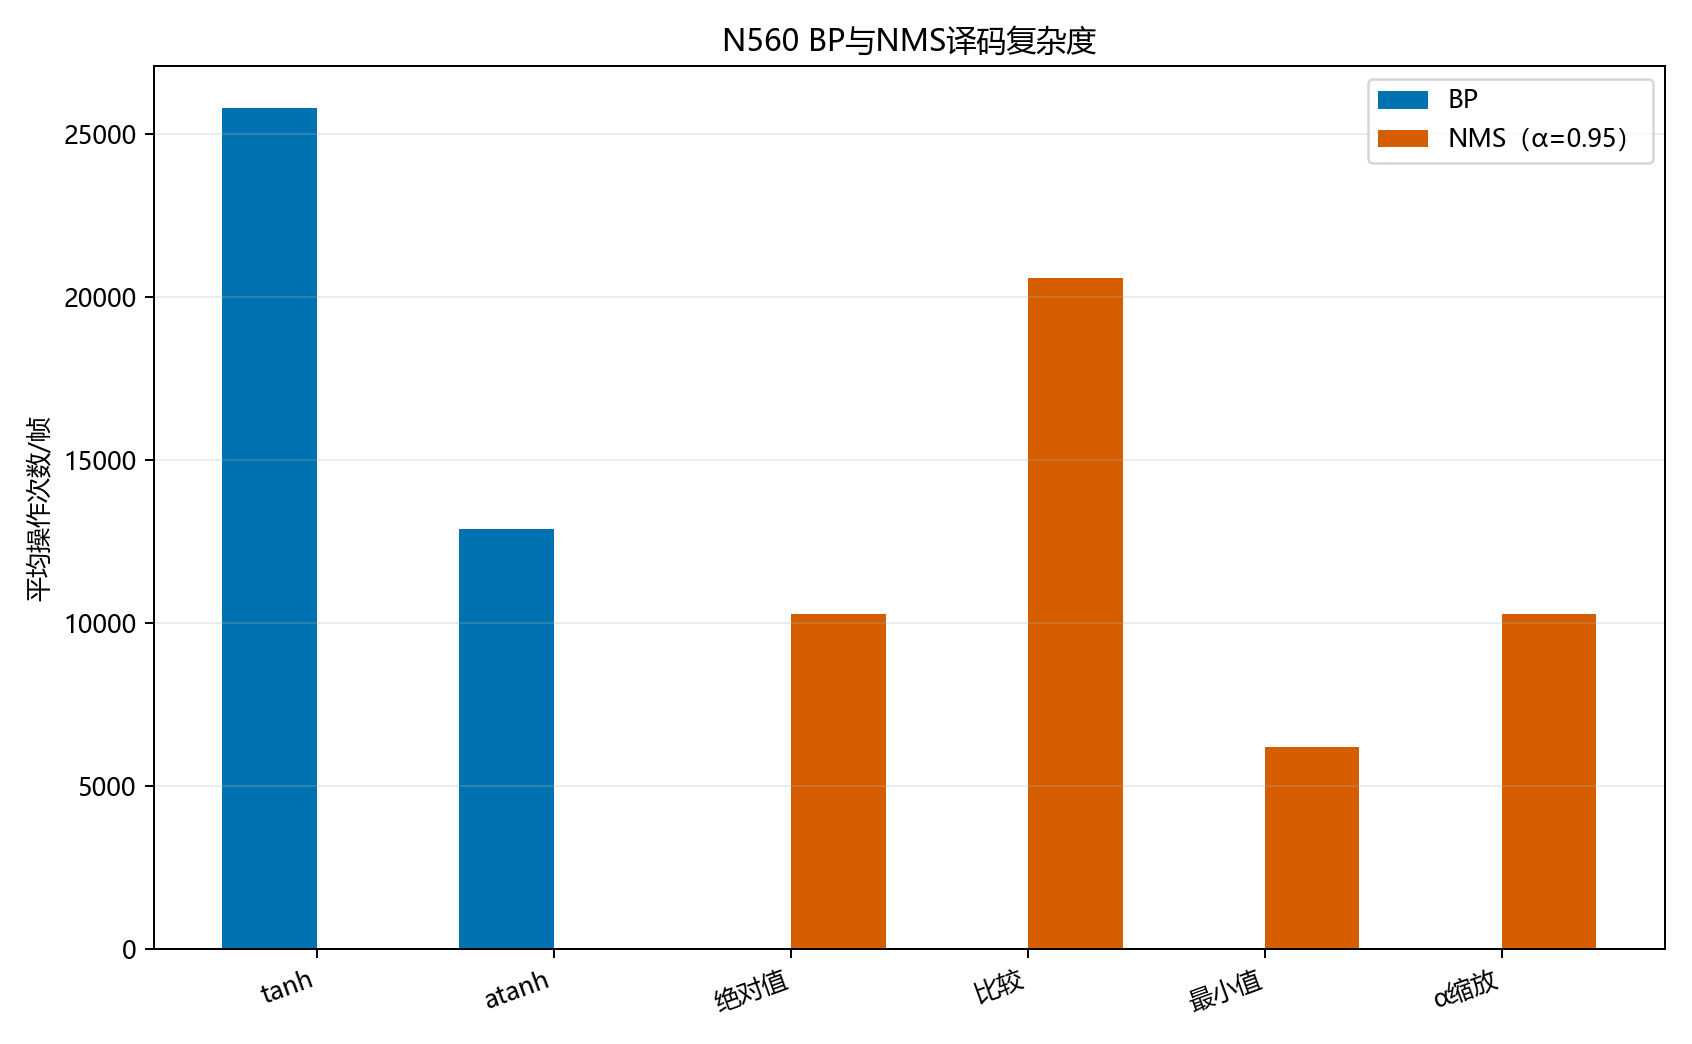
\includegraphics[width=0.98\linewidth]{../Task/Comparison/S6/results/summary/figures/ldpc_05_complexity/figure.png}\\[-0.2em]\small（a）主要操作结构
  \end{minipage}\hfill
  \begin{minipage}{0.49\textwidth}\centering
    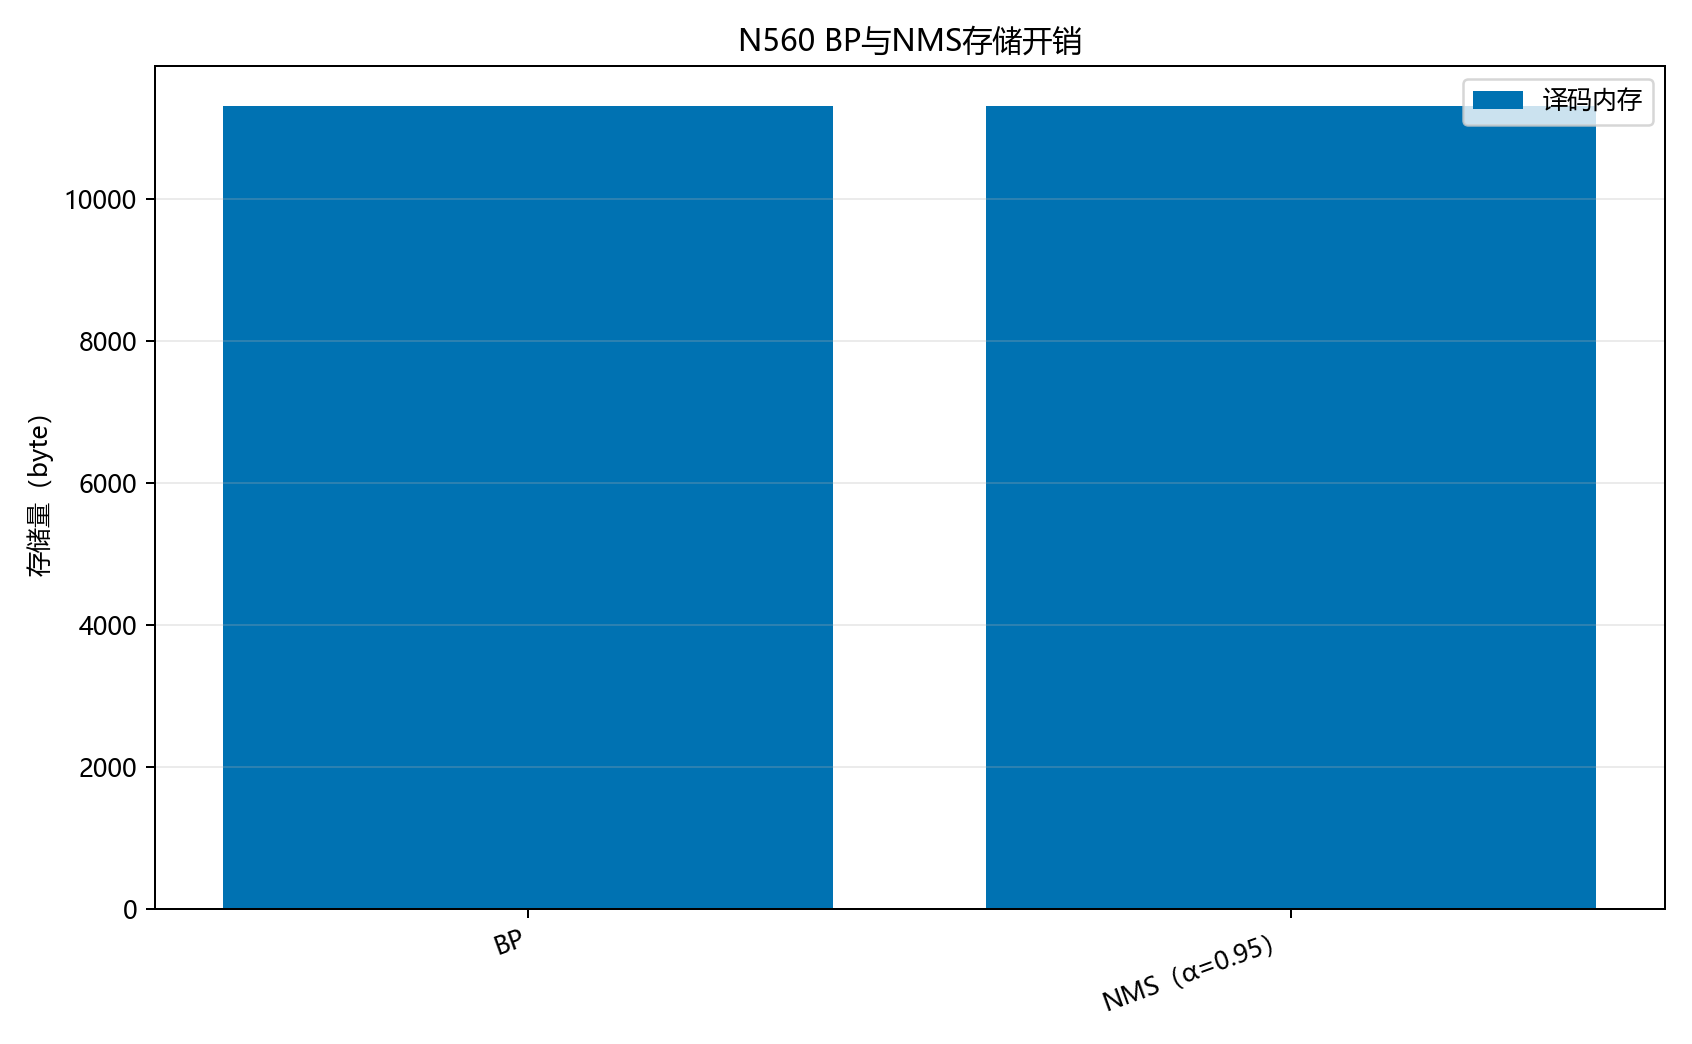
\includegraphics[width=0.98\linewidth]{../Task/Comparison/S6/results/summary/figures/ldpc_06_memory/figure.png}\\[-0.2em]\small（b）译码器内存
  \end{minipage}\par\medskip
  \begin{minipage}{0.49\textwidth}\centering
    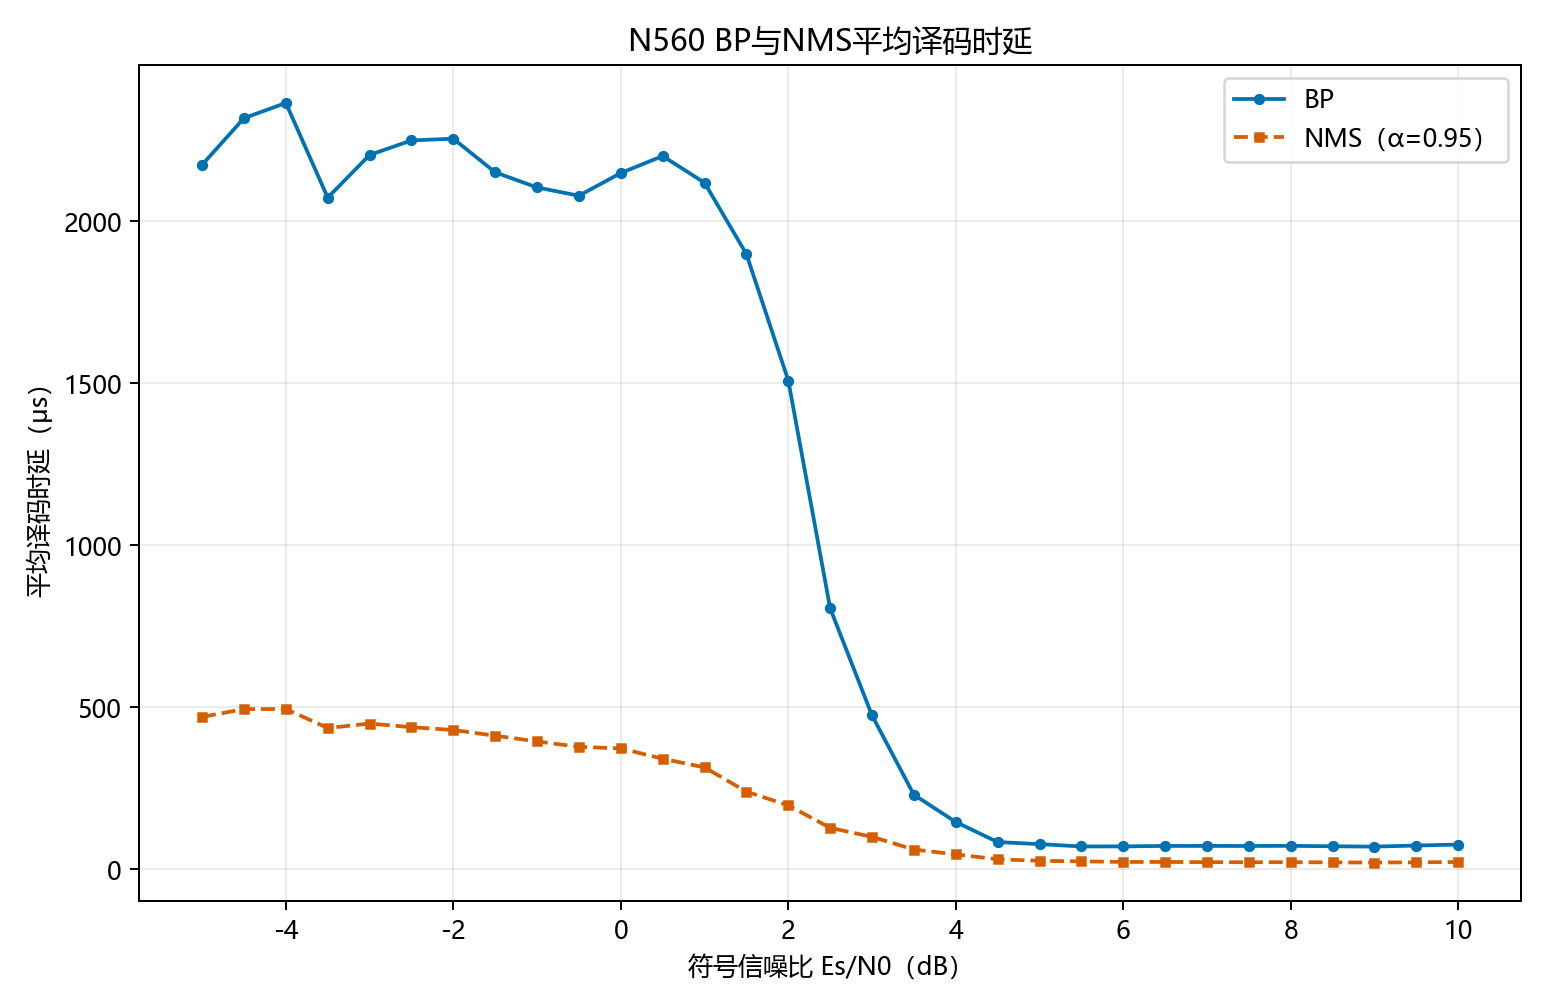
\includegraphics[width=0.98\linewidth]{../Task/Comparison/S6/results/summary/figures/ldpc_07_avg_time/figure.png}\\[-0.2em]\small（c）平均译码时间
  \end{minipage}\hfill
  \begin{minipage}{0.49\textwidth}\centering
    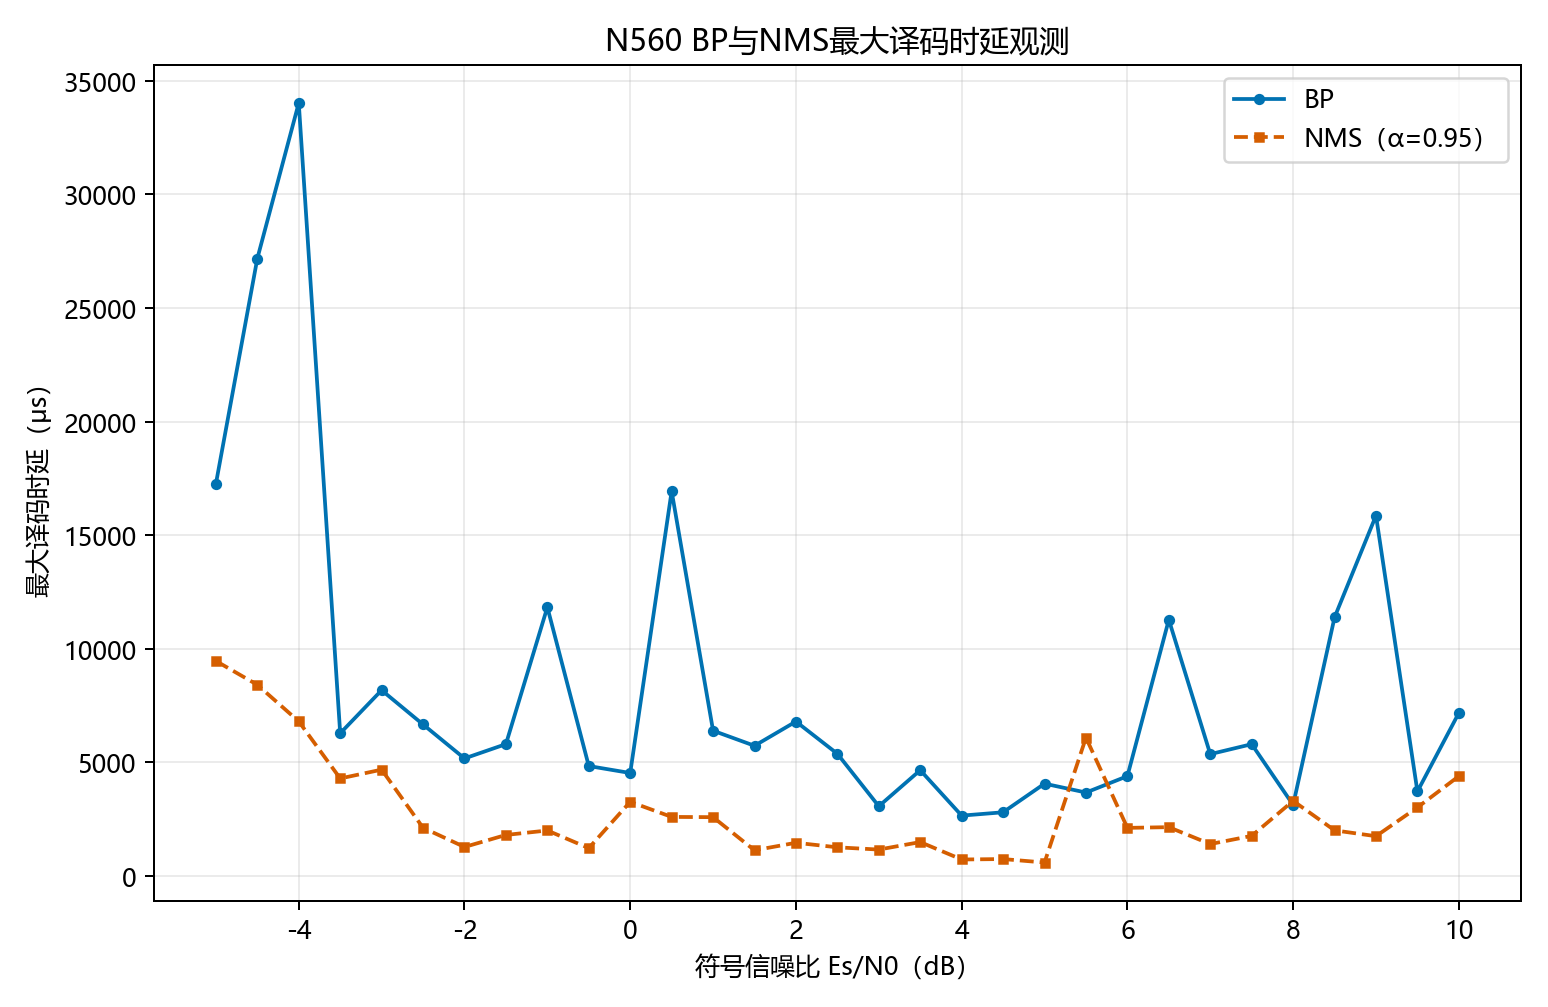
\includegraphics[width=0.98\linewidth]{../Task/Comparison/S6/results/summary/figures/ldpc_08_max_time/figure.png}\\[-0.2em]\small（d）最大观测译码时间
  \end{minipage}
  \caption{LDPC BP与NMS的计算结构、存储和软件时间}
  \label{fig:s6-ldpc-cost}
\end{figure}

\begin{table}[htbp]
  \centering
  \scriptsize
  \caption{LDPC BP与NMS的可靠性、复杂度和时间指标}
  \label{tab:s6-ldpc-summary}
  \setlength{\tabcolsep}{2.0pt}
  \begin{tabular}{p{0.08\textwidth}cccccc p{0.18\textwidth}}
    \toprule
    译码器 & FER=0.1/dB & FER=0.01/dB & 网格平均迭代 & 加权平均/$\mu$s & 最大/$\mu$s & 内存/byte & 校验节点主要运算 \\
    \midrule
    BP & 4.541 & 5.866 & 16.44 & 140.687 & 34024.9 & 11312 & 双曲正切、反双曲正切、消息更新 \\
    NMS & 4.577 & 5.875 & 13.11 & 33.157 & 9468.0 & 11312 & 绝对值、比较、最小值、符号和缩放 \\
    \bottomrule
  \end{tabular}
\end{table}

\subsection{LDPC工程结论}

BP提供当前实现的可靠性基准，其非线性校验节点更新带来较高软件计算代价。NMS以最小值近似和归一化系数简化校验节点更新，在FER为0.1和0.01时仅损失0.036 dB和0.010 dB，同时将加权平均和最大观测软件译码时间分别降低76.4\%和72.2\%，且不增加模型内存。对于本项目N560、$\alpha=0.95$和32次迭代上限的配置，NMS形成了可靠性损失很小而软件时间明显下降的工程替代；该判断不外推到其他码长、系数或硬件实现。

\section{三类译码实现的工程特征综合}

表\ref{tab:s6-engineering-summary}按编码族总结可靠性、计算、存储与时间特征，不建立跨族BER或操作计数排名。三类任务的载荷、码长、图结构和操作语义不同，BCH的一次有限域乘法、Viterbi的一次ACS与LDPC的一次比较不具有统一成本。软件时间和模型内存虽然使用共同单位，也只反映当前软件环境和各自计时、建模范围，不能直接替代目标硬件评估。

\begin{table}[htbp]
  \centering
  \scriptsize
  \caption{三类译码实现的工程特征汇总}
  \label{tab:s6-engineering-summary}
  \setlength{\tabcolsep}{1.7pt}
  \begin{tabular}{p{0.07\textwidth}p{0.12\textwidth}p{0.13\textwidth}p{0.15\textwidth}p{0.11\textwidth}p{0.12\textwidth}p{0.11\textwidth}}
    \toprule
    编码族 & 译码器 & 可靠性特征 & 主要计算结构 & 存储特征 & 软件时间特征 & 适用倾向 \\
    \midrule
    BCH & 分组查表 & 当前完整方案门限较高 & 短综合征、查表、翻转 & 固定表与小工作区 & 平均时间较低 & 结构固定、资源受限 \\
    BCH & BM与Chien & 当前完整方案门限降低 & 综合征、BM、Chien、有限域运算 & 有限域表与代数状态增加 & 平均时间增加 & 整块纠错能力优先 \\
    卷积码 & 硬判决Viterbi & 损失幅值可靠性信息 & 汉明度量、ACS、回溯 & 与同组织软判决相同 & 分支度量较轻 & 资源或实时性优先 \\
    卷积码 & 浮点软判决Viterbi & FER门限改善约2.1--2.3 dB & 欧氏度量、ACS、回溯 & 与同组织硬判决相同 & CPU时间增加 & 可靠性优先 \\
    LDPC & 分层BP & 可靠性基准 & 非线性校验节点和消息更新 & 消息缓冲11312 byte & 当前实现较慢 & 性能基准与高精度实现 \\
    LDPC & 分层NMS & 门限损失不超过0.04 dB & 最小值、符号和归一化 & 消息缓冲11312 byte & 平均时间降低76.4\% & 低复杂度软件实现 \\
    \bottomrule
  \end{tabular}
\end{table}

从同族选择看，BCH需要在短分组查表的低实现代价与整块代数方案的纠错收益之间权衡；卷积码需要在软信息带来的约2 dB可靠性收益与分支度量开销之间权衡；LDPC则体现出NMS以很小门限损失换取显著软件加速的特点。工程选型应把BER、FER、操作结构、存储、平均时间和最大观测时间同时纳入，而不是只根据一条误码曲线作结论。

\section{本章结论}

BCH比较表明，分组综合征查表适合短分组和固定结构，BCH-S200以较小内存和较低软件时间完成译码；BM与Chien搜索适合较长整块BCH，BCH-B200在FER为0.01时节省1.671 dB，但平均译码时间和模型内存分别增加70.5\%和52.4\%。该BER/FER差异属于两套完整方案的综合差异，不能纯归因于译码器。

卷积码比较表明，浮点软判决保留连续接收幅值的可靠性信息，在FER为0.1和0.01时相对硬判决分别获得2.098 dB和2.260 dB收益；代价是整块加权平均CPU译码时间增加54.6\%，分支度量需要浮点减法、平方和加法。硬判决适合计算精度与实时资源更紧、同时链路余量允许可靠性损失的场景。连续方案的首输出和决策时延属于符号调度指标，不能与CPU墙钟时间混称。

LDPC比较表明，BP是当前N560配置的性能基准，NMS通过最小值、符号和$\alpha=0.95$缩放替代非线性校验节点计算。NMS在两个目标FER处的损失均小于0.04 dB，加权平均和最大观测软件译码时间分别降低76.4\%和72.2\%，模型内存保持不变。复杂度判断必须同时考虑单次迭代结构与实际迭代次数。

三类结果共同说明，译码器选择需要同时满足可靠性、计算复杂度、存储和实时性约束。误码曲线回答链路余量问题，操作计数揭示实现结构，平均时间描述常态软件负担，最大观测时间暴露尾部风险；只有在保持各指标定义与比较边界的前提下，才能形成可追溯的工程选择。
